\documentclass[10pt]{article}
\linespread{.7}
\usepackage[a4paper, margin=3mm, landscape]{geometry}
\usepackage{multicol}
\usepackage{xcolor}
\usepackage{enumitem}
\usepackage{amsmath}
\usepackage{amsfonts}
\usepackage{listings}
\usepackage{soul}
\usepackage{graphicx}

\pdfinfo{
    /Title (ACC1701x.pdf)
    /Creator (TeX)
    /Producer (pdfTeX 1.40.0)
    /Author (Vincent Pang)
    /Subject (CS2106)
    /Keywords (CS2106, nus, cheatsheet, pdf)
}

\graphicspath{ {./img/} }

\pagestyle{empty}
\setcounter{secnumdepth}{0}
\setlength{\columnseprule}{0.25pt}

% Redefine section commands to use less space
\makeatletter
\renewcommand{\section}{\@startsection{section}{1}{0mm}%
    {-1ex plus -.5ex minus -.2ex}%
    {0.5ex plus .2ex}%x
{\normalfont\large\bfseries}}
\renewcommand{\subsection}{\@startsection{subsection}{2}{0mm}%
    {-1explus -.5ex minus -.2ex}%
    {0.5ex plus .2ex}%
{\normalfont\normalsize\bfseries}}
\renewcommand{\subsubsection}{\@startsection{subsubsection}{3}{0mm}%
    {-1ex plus -.5ex minus -.2ex}%
    {1ex plus .2ex}%
{\normalfont\small\bfseries}}%
\makeatother

% Adjust spacing for all itemize/enumerate
\setlength{\leftmargini}{0.5cm}
\setlength{\leftmarginii}{0.5cm}
\setlist[itemize,1]{leftmargin=2mm,labelindent=1mm,labelsep=1mm}
\setlist[itemize,2]{leftmargin=2mm,labelindent=1mm,labelsep=1mm}

% Font
\renewcommand{\familydefault}{\sfdefault}

% Define colors for math formulas
\definecolor{myblue}{cmyk}{1,.72,0,.38}
\everymath\expandafter{\the\everymath \color{myblue}}

% Custom command for keywords
\definecolor{highlight}{RGB}{251,243,218}
\newcommand{\keyword}[2][]{\sethlcolor{highlight}\hl{\textbf{#2}} #1 - }
\newcommand{\ilkeyword}[1]{\sethlcolor{highlight}\hl{\textbf{#1}}}

% Define colors and style for code
\definecolor{codegreen}{rgb}{0,0.6,0}
\definecolor{codegray}{rgb}{0.5,0.5,0.5}
\definecolor{codered}{HTML}{CC241D}
\definecolor{backcolor}{rgb}{0.95,0.95,0.95}
\lstdefinestyle{codestyle}{
    backgroundcolor = \color{backcolor},
    commentstyle = \color{codegray},
    keywordstyle = \color{codered},
    stringstyle = \color{codegreen},
    basicstyle = \ttfamily,
    breakatwhitespace = false,
    showstringspaces = false,
    breaklines = true,
    showtabs = false,
    tabsize = 2
}
\lstset{style = codestyle}

% -----------------------------------------------------------------------
\begin{document}
\begin{multicols*}{3}
\footnotesize

% Title box
\begin{center}
    \fbox{
        \parbox{0.8\linewidth}{
            \centering \textcolor{black}{
                {\Large\textbf{CS2106}} \\
                \normalsize{AY22/23 Sem 2}} \\
                {\footnotesize \textcolor{gray}{github.com/securespider}}
        }
    }
\end{center}
\section{01. Introduction}
\keyword{OS}{Program that acts as an intermediary between user and hardware}

\subsection{Different architectures}
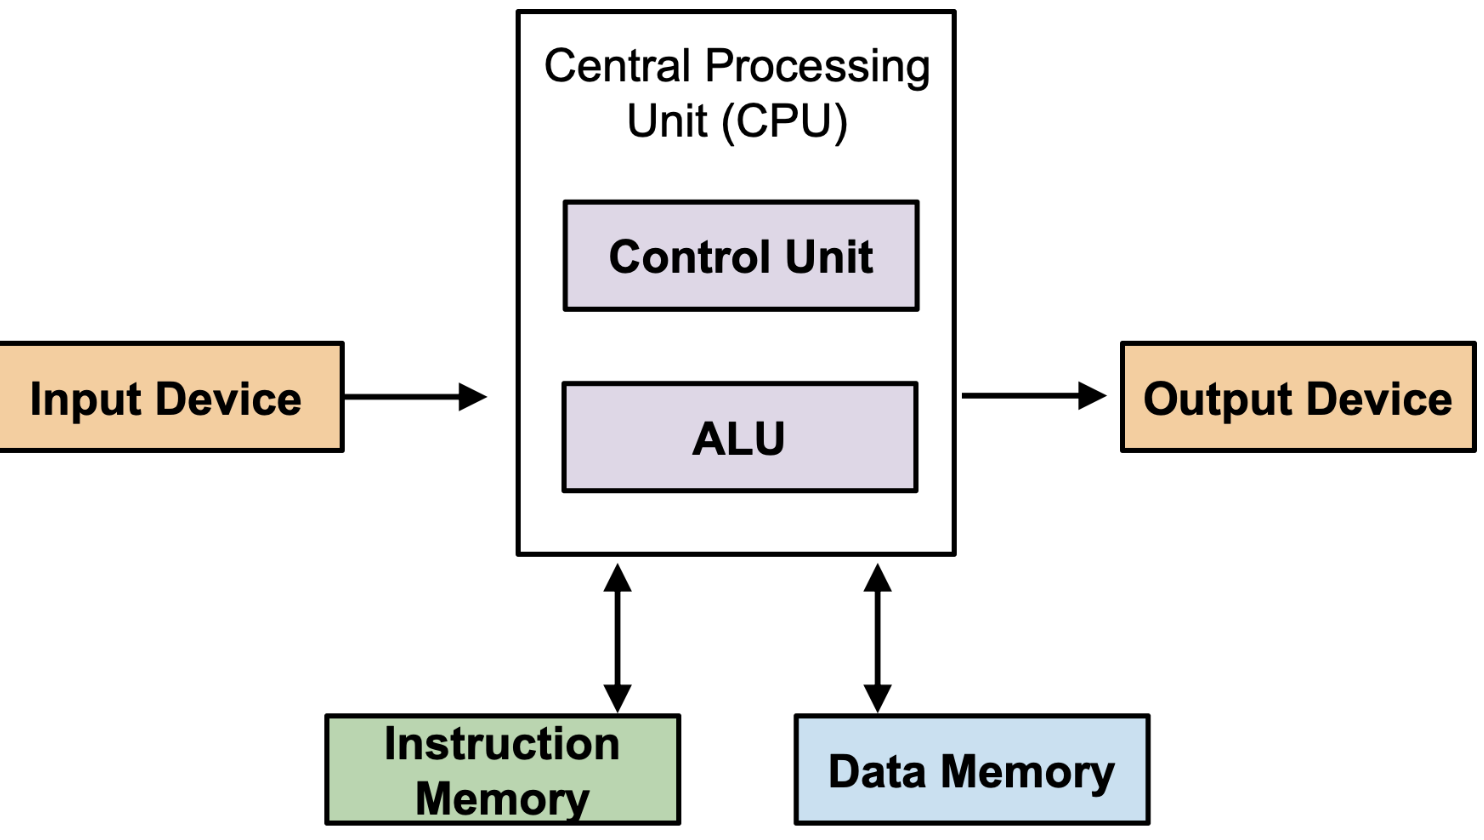
\includegraphics[scale=0.17]{harvard-architecture}
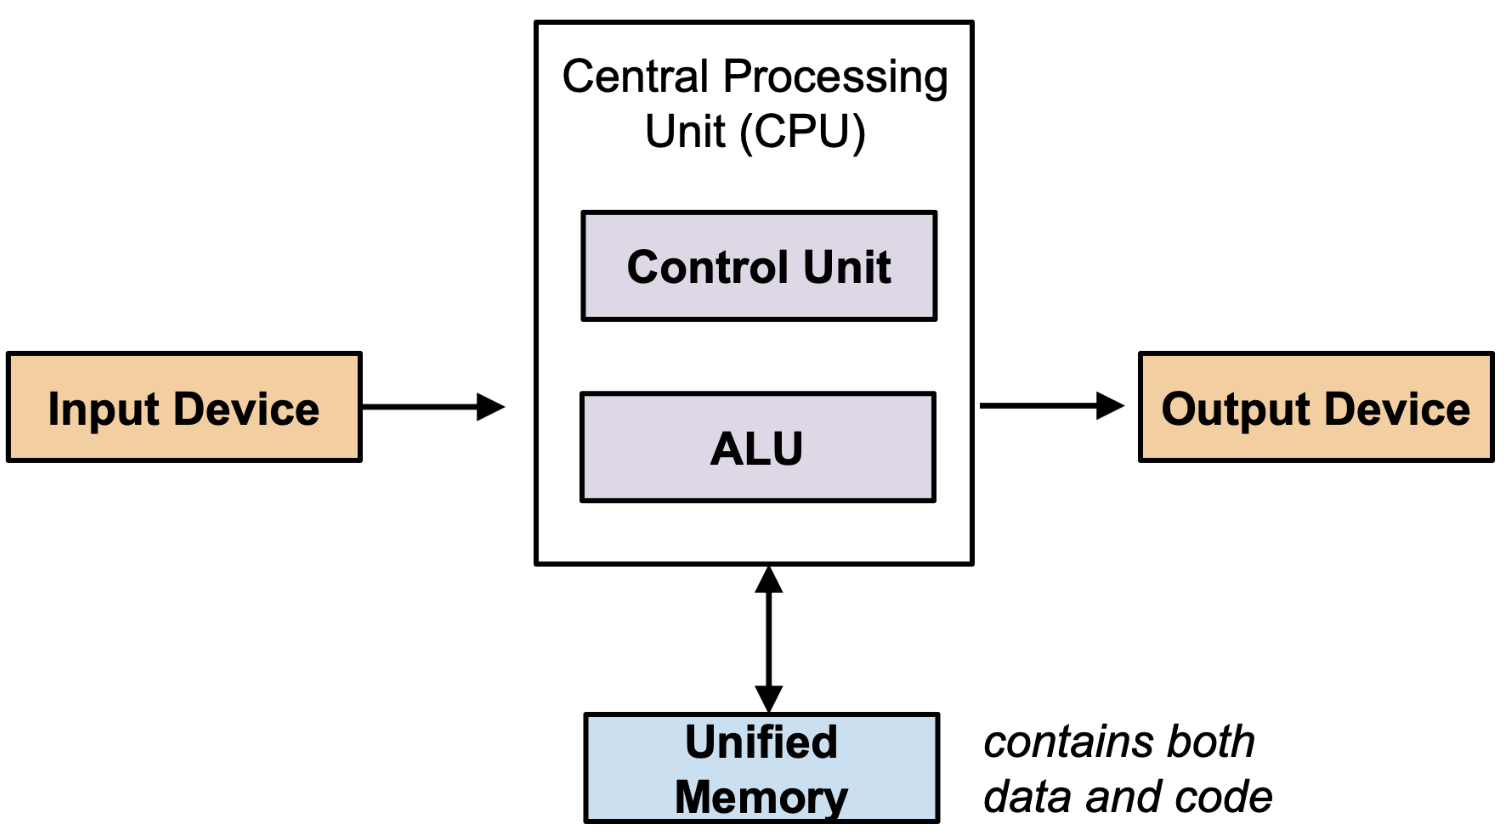
\includegraphics[scale=0.17]{von-neumann}

\begin{description}
	\item[Difference]{Separate vs common storage pathway for code and data}
\end{description}
Why do we need OS?
\begin{itemize}
	\item Should not have bugs
	\item Treat process as malicious
\end{itemize}

\subsection{Mainframe}
Old analog "computers" using physical cards for programming
\subsubsection{Improvements}
\begin{itemize}
	\item Problem: Batch processing inefficient
	\item Solution: Multiprogramming
	\begin{itemize}
		\item Loading multiple jobs that runs while other jobs using I/O
		\item Overlapping computation with I/O
	\end{itemize}
	\item Problem: Only one user 
	\item Solution: Time sharing OS
	\begin{itemize}
		\item Multiple concurrent users using terminals
		\item User job scheduling 
		\item Memory management
		\item \keyword{Hardware virtualization}{Each program executes as if it had all resources}
	\end{itemize}
\end{itemize}


\subsection{Motivation}
\begin{enumerate}
	\item Abstraction
	\begin{itemize}
		\item Hide low level details and present common, high-level functionality to users
	\end{itemize}
	\item Resource allocation
	\begin{itemize}
		\item Allow concurrent usage of resource and execute programs simultaneously
		\item Arbitrate conflicting request fairly and efficiently
	\end{itemize}
	\item Control programs
	\begin{itemize}
		\item Restrict resource allocation
		\item Security, protection and error prevention (Defensive)
		\item Ensure proper use of device
	\end{itemize}
\end{enumerate}
\subsubsection{Advantage}
\begin{itemize}
	\item Portable and flexible
	\item Use computer resources efficiently
\end{itemize}
\subsubsection{Disadvantage}
\begin{itemize}
	\item Significant overhead
\end{itemize}

\subsubsection{OS vs User Program}
Similarities
\begin{itemize}
	\item Both softwares
\end{itemize}
Difference
\begin{itemize}
	\item OS runs in \keyword{kernel mode}{Access to all hardware resources}
	\item User programs run in \keyword{User mode}{Limited access}
	\item User programs use syscalls to communicate with OS for hardware processes
	\item User - Full virtual address space for code but cannot write outside of virtual address space
	\item Kernel - All code share same address space
\end{itemize}
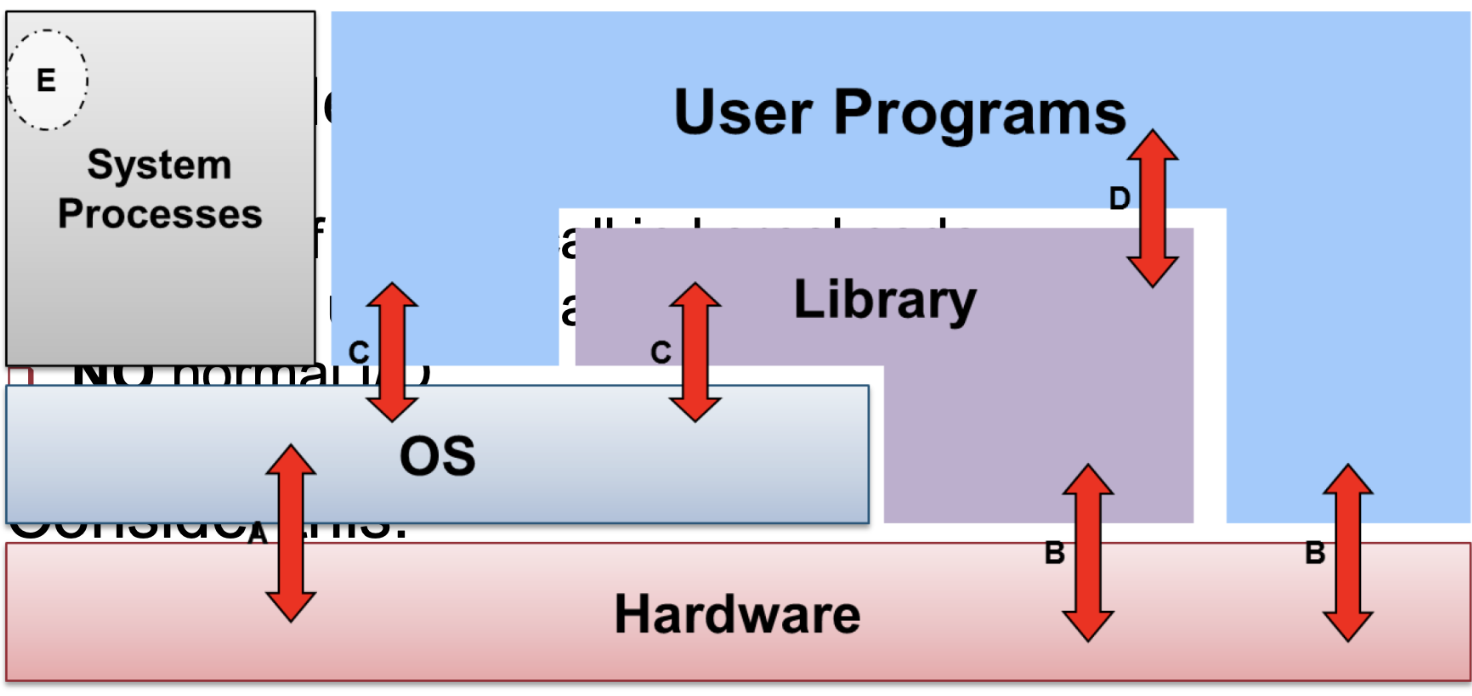
\includegraphics[scale=0.28]{os-interaction}
\begin{description}
	\item[A]{OS executes machine instructions}
	\item[B]{Normal machine instructions executed}
	\item[C]{Calling OS using \textbf{syscall interface}}
	\item[D]{User programs call library code}
	\item[E]{System processes providing high level services}
\end{description}
Why OS dont occupy entire hardware layer
\begin{itemize}
	\item Slow to have all operations pass through intermediary
	\item User programs can have direct interaction with hardware (eg. Arithmetic) during low risk operations
\end{itemize}

\subsection{OS structure}
\subsubsection{Monolithic OS}
\begin{itemize}
	\item One big kernel program
	\item Well understood and has good performance
	\item Highly \keyword{coupled}{internal structure interconnected that unintentionally affect each other}
\end{itemize}
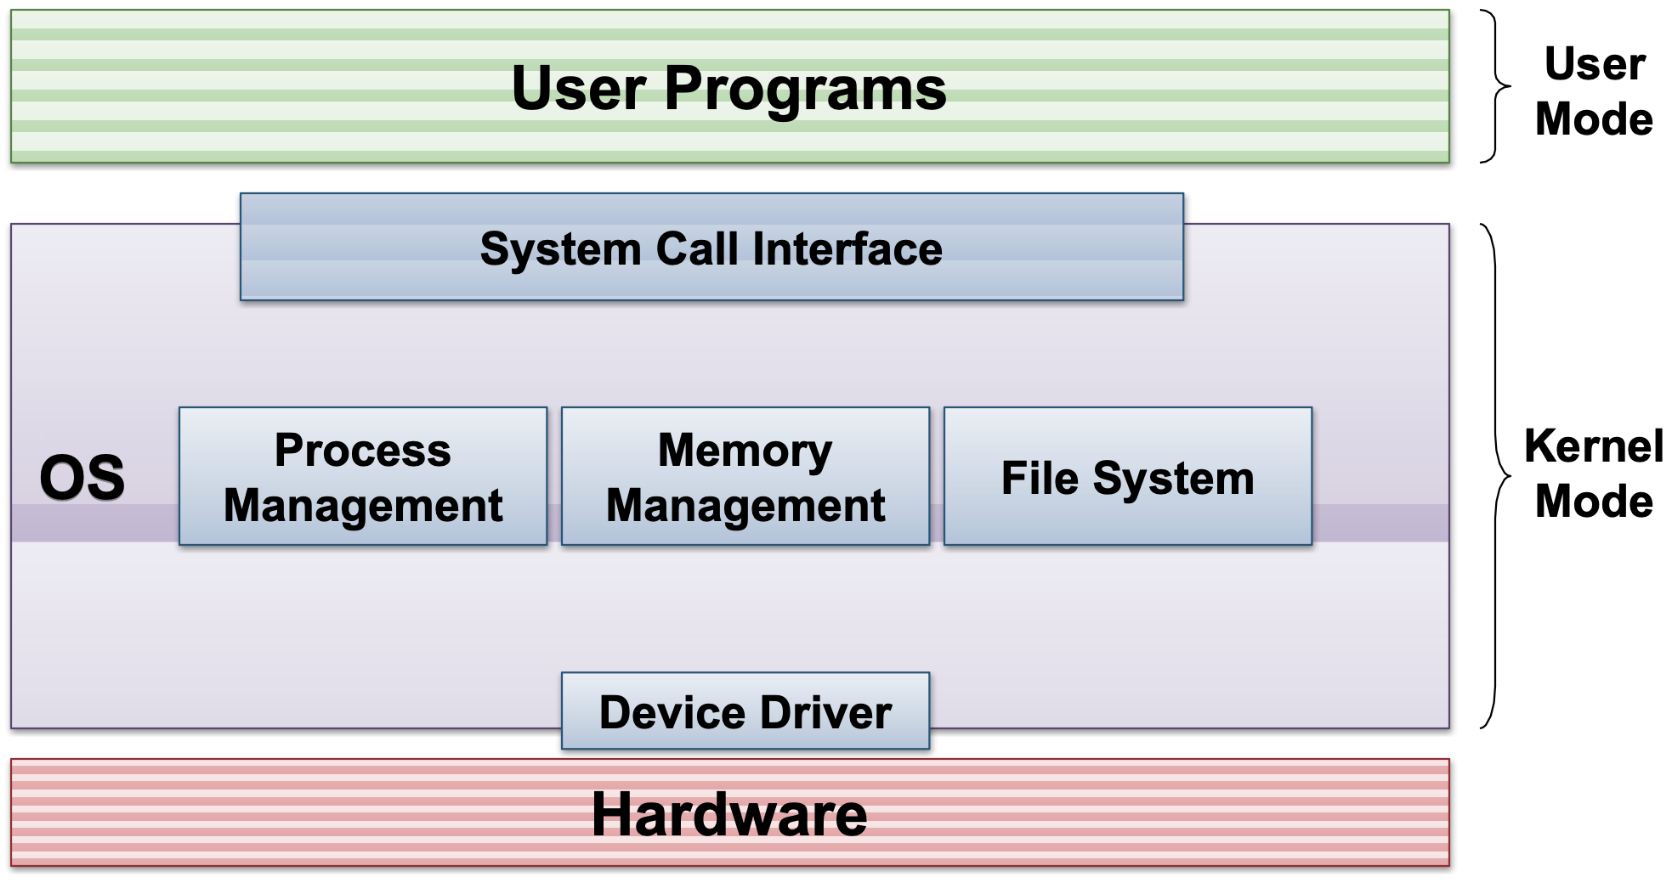
\includegraphics[scale=0.25]{monolithic-os}

\subsubsection{Microkernel}
\begin{itemize}
	\item Small clean
	\item Basic and essential facilities
	\item IPC communication OR run external programs outside OS
	\item Robust and more \keyword{modular}{Extendible and maintainable}
	\item Better isolation btw kernel and services
	\item Lower performance
	\item Unix is monolithic kernel, Windows is hybrid 
\end{itemize}
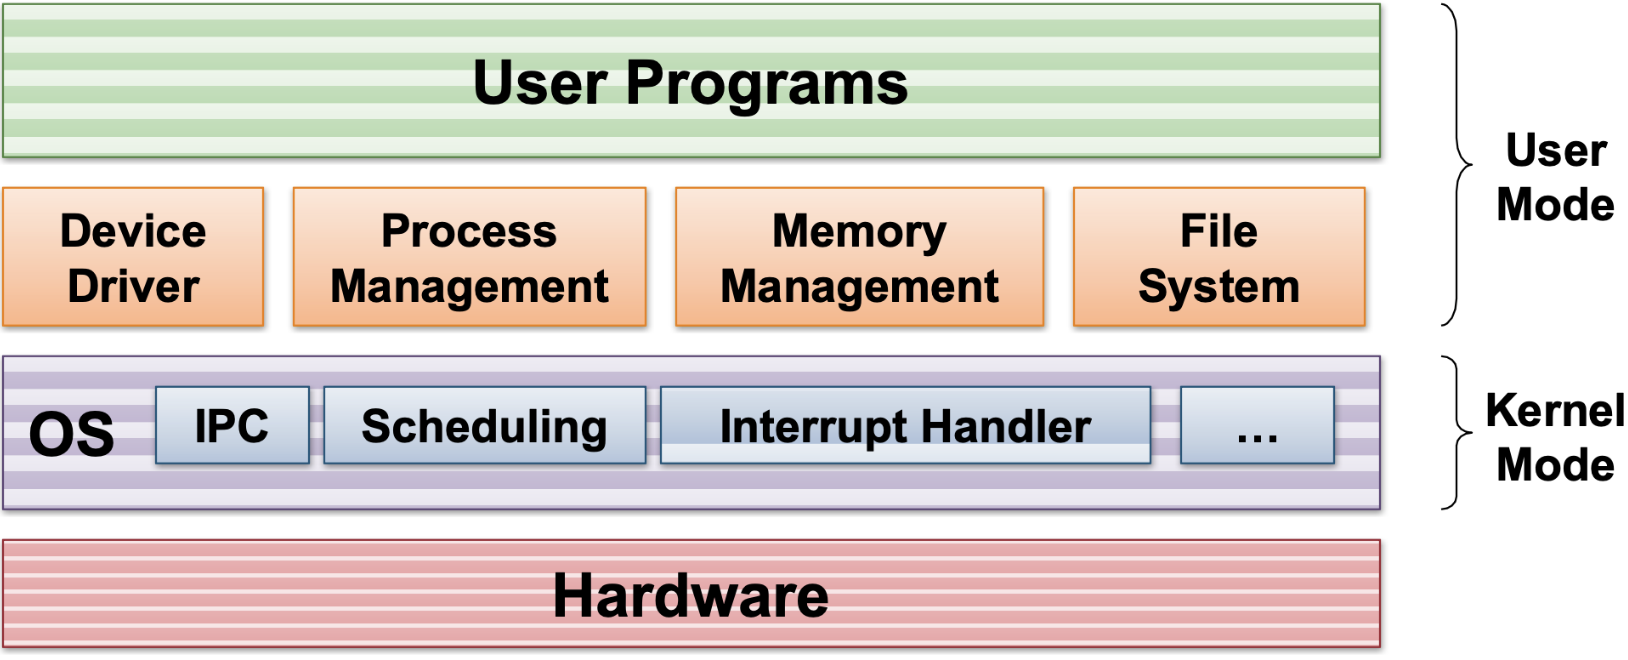
\includegraphics[scale=0.28]{microkernel-os}
\subsection{Virtual Machines}
\begin{itemize}
	\item Software emulation of hardware
	\item Virtualization of underlying hardware to run additional operating systems concurrently
\end{itemize}
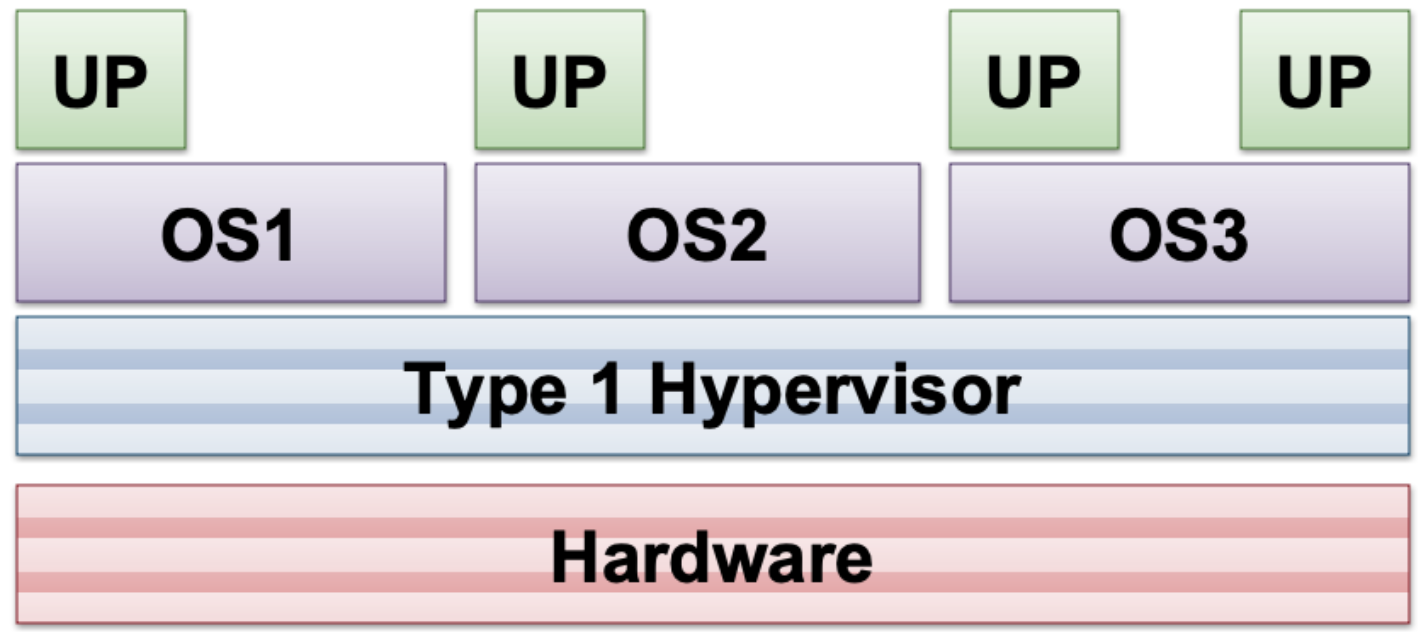
\includegraphics[scale=0.2]{type-1-hypervisor}
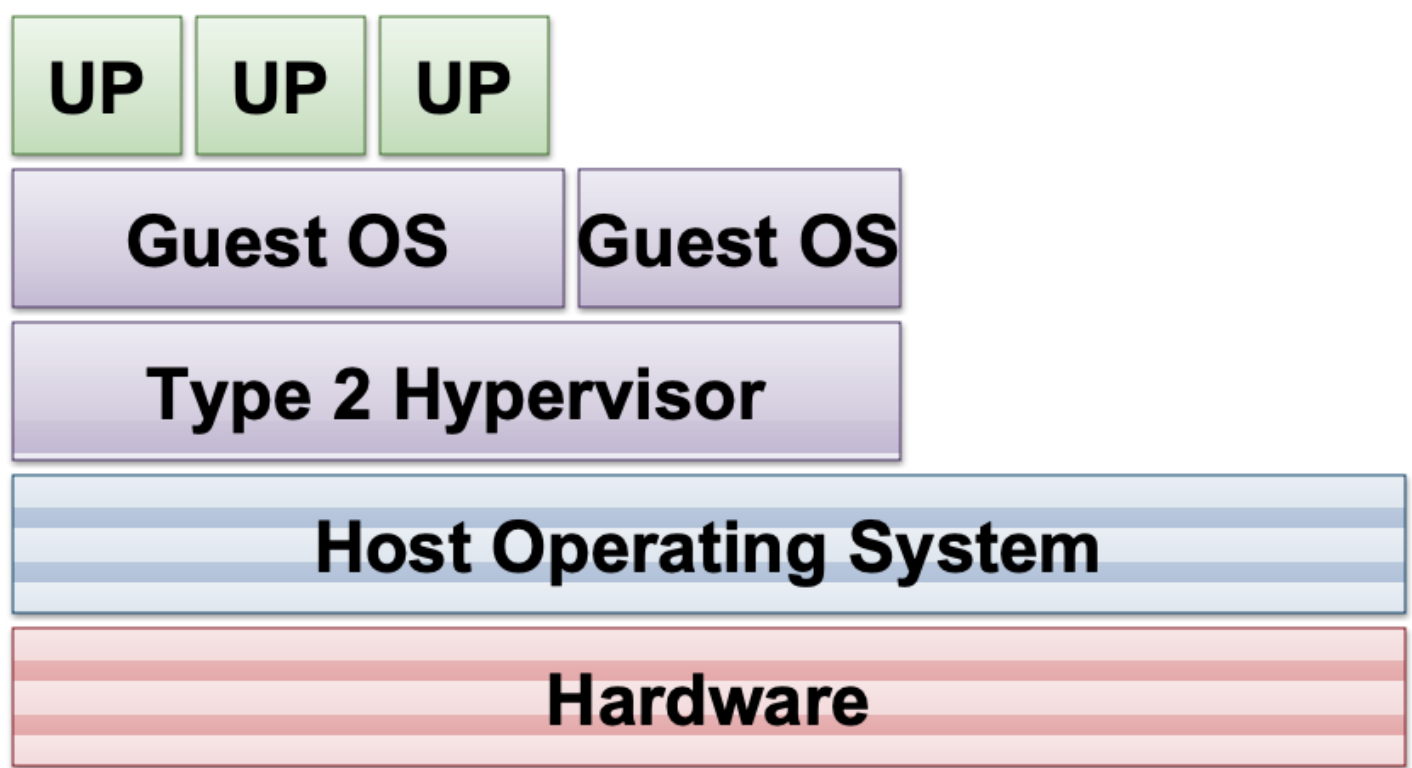
\includegraphics[scale=0.2]{type-2-hypervisor}

%--------------------------------------------------------------------------------------------------------------------

\section{02. Process abstraction}
\subsection{Motivation}
\begin{itemize}
	\item Allow concurrent usage of hardware
	\item Multiple programs sharing the same processors/IO
\end{itemize}
\subsection{Computer organisation}
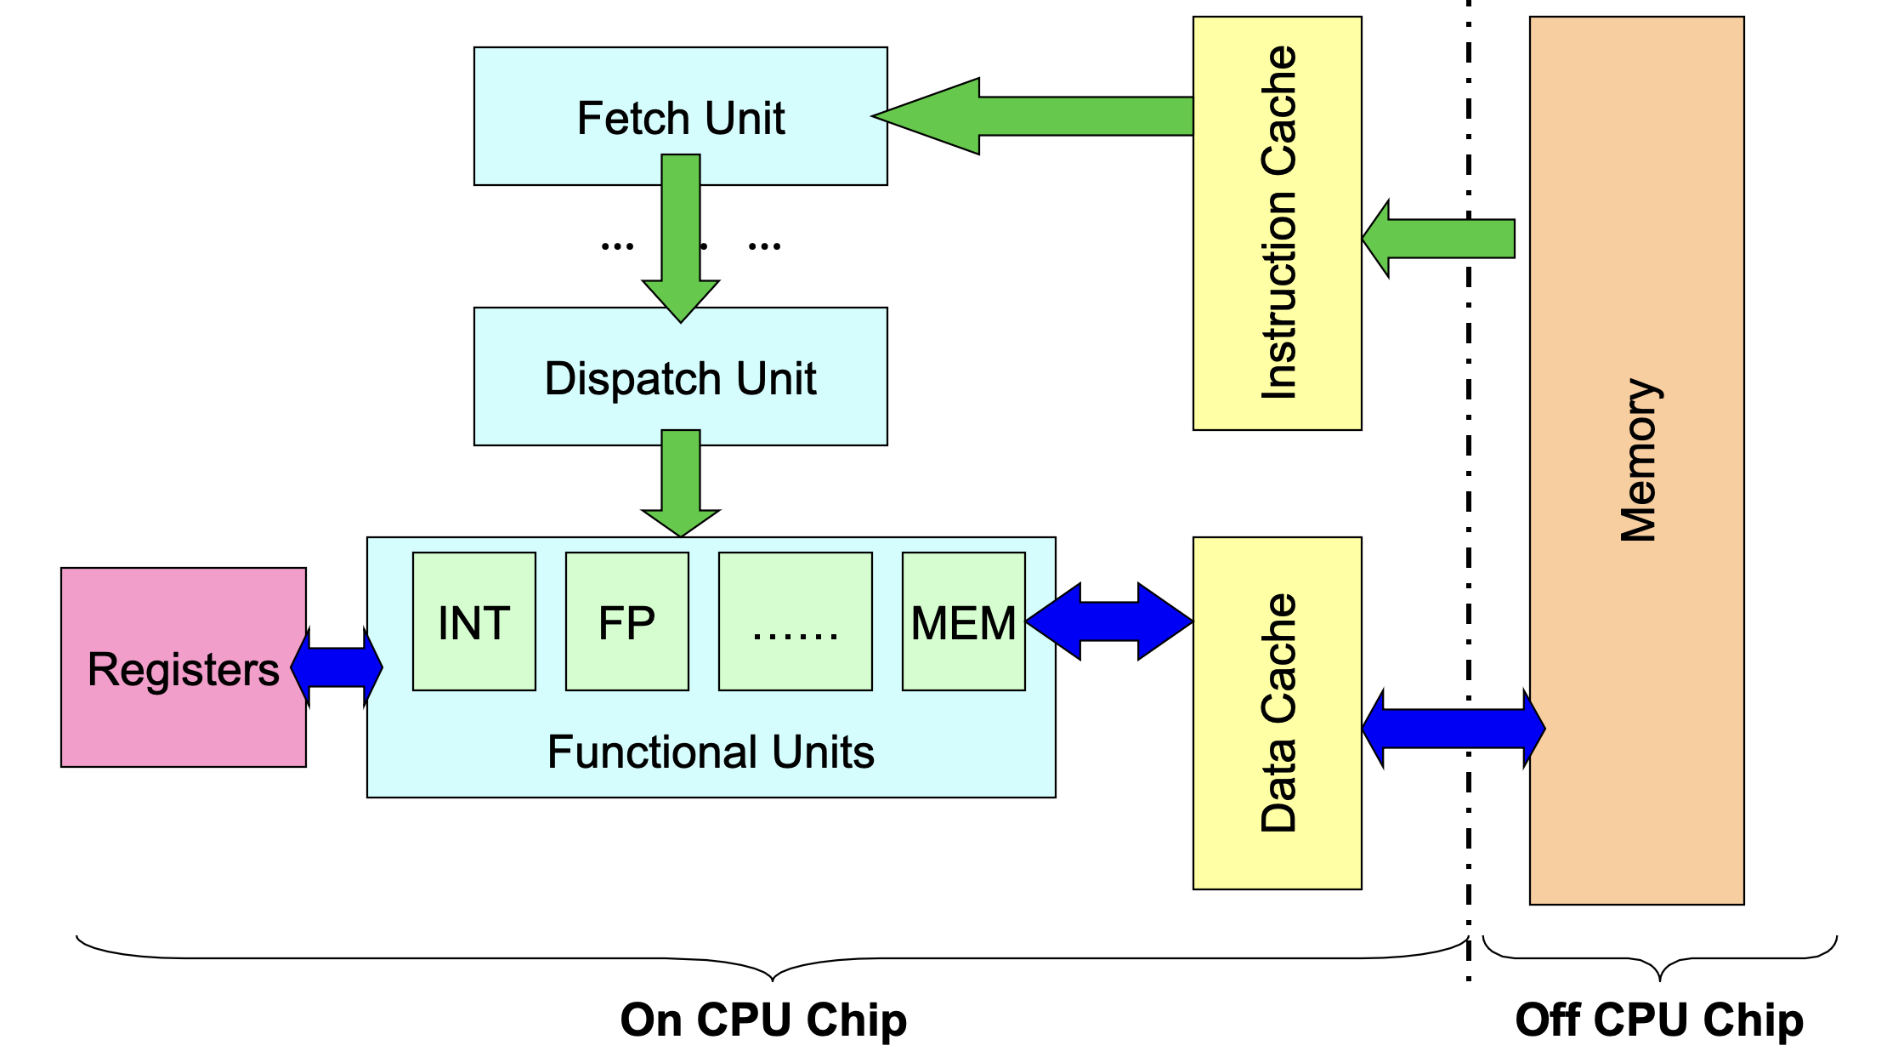
\includegraphics[scale=0.27]{computer-organisation}
\subsubsection{Memory}
\begin{itemize}
	\item Storage for instruction and data
	\item Managed by the OS
	\item Normally accessed via load/store instructions
\end{itemize}
\subsubsection{Cache}
\begin{itemize}
	\item Fast and invisible to software
	\item Duplicate part of the memory for faster access
	\item Usually split into instruction and data cache
\end{itemize}
\subsubsection{Fetch}
\begin{itemize}
	\item Load instructions from memory
	\item Location indicated by \textbf{Program Counter}
\end{itemize}
\subsubsection{Functional units}
\begin{itemize}
	\item Carry out instruction execution
	\item Dedicated to specific instruction type
\end{itemize}
\end{multicols*}
\begin{multicols*}{4}
\subsubsection{Registers}
\begin{itemize}
	\item Internal storage for fastest access speed
\end{itemize}
\subsection{Information needed}
\begin{itemize}
	\item Memory context
	\begin{itemize}
		\item Code
		\item Data
	\end{itemize}
	\item Hardware context
	\begin{itemize}
		\item Register
		\item PC value
		\item Frame Pointer
	\end{itemize}
	\item OS context
	\begin{itemize}
		\item Process properties
		\item Resources used
		\item Files
	\end{itemize}
\end{itemize}

\subsection{Function calls}
Suppose a function f() calls g()
\begin{itemize}
	\item f is caller and g is callee
\end{itemize}
Steps of control flow
\begin{enumerate}
	\item Setup parameters
	\item Trf ctrl to callee
	\item Setup local var
	\begin{itemize}
		\item Remember the initial variables especially if registers are to be reverted back when jumping back to caller
		\item Callee does not know the registers callers used, so prevent accidental overwrite of content to registers caller use
	\end{itemize}
	\item Store any results
	\item Return ctrl to caller
\end{enumerate}
\subsubsection{Issues}
Control Flow
\begin{itemize}
	\item Need to jump to functional body when callee called
	\item Need to resume to next instruction in caller after done
\end{itemize}
Data storage
\begin{itemize}
	\item Need to pass parameters to function
	\item Need to capture return result
	\item May have local variables
\end{itemize}
Additional
\begin{itemize}
	\item May lead to overriding of data in caller by callee (interference)
	\item Calling g() multiple times may lead to insufficient space and overriding
\end{itemize}


\subsection{Stack memory}
Memory to store function invocation\\
\keyword{Stack Pointer}{Indicates the first free location in the stack region}\\
\keyword{Frame Pointer}{Points to the frame and is used for traversing around the stack easily}\\
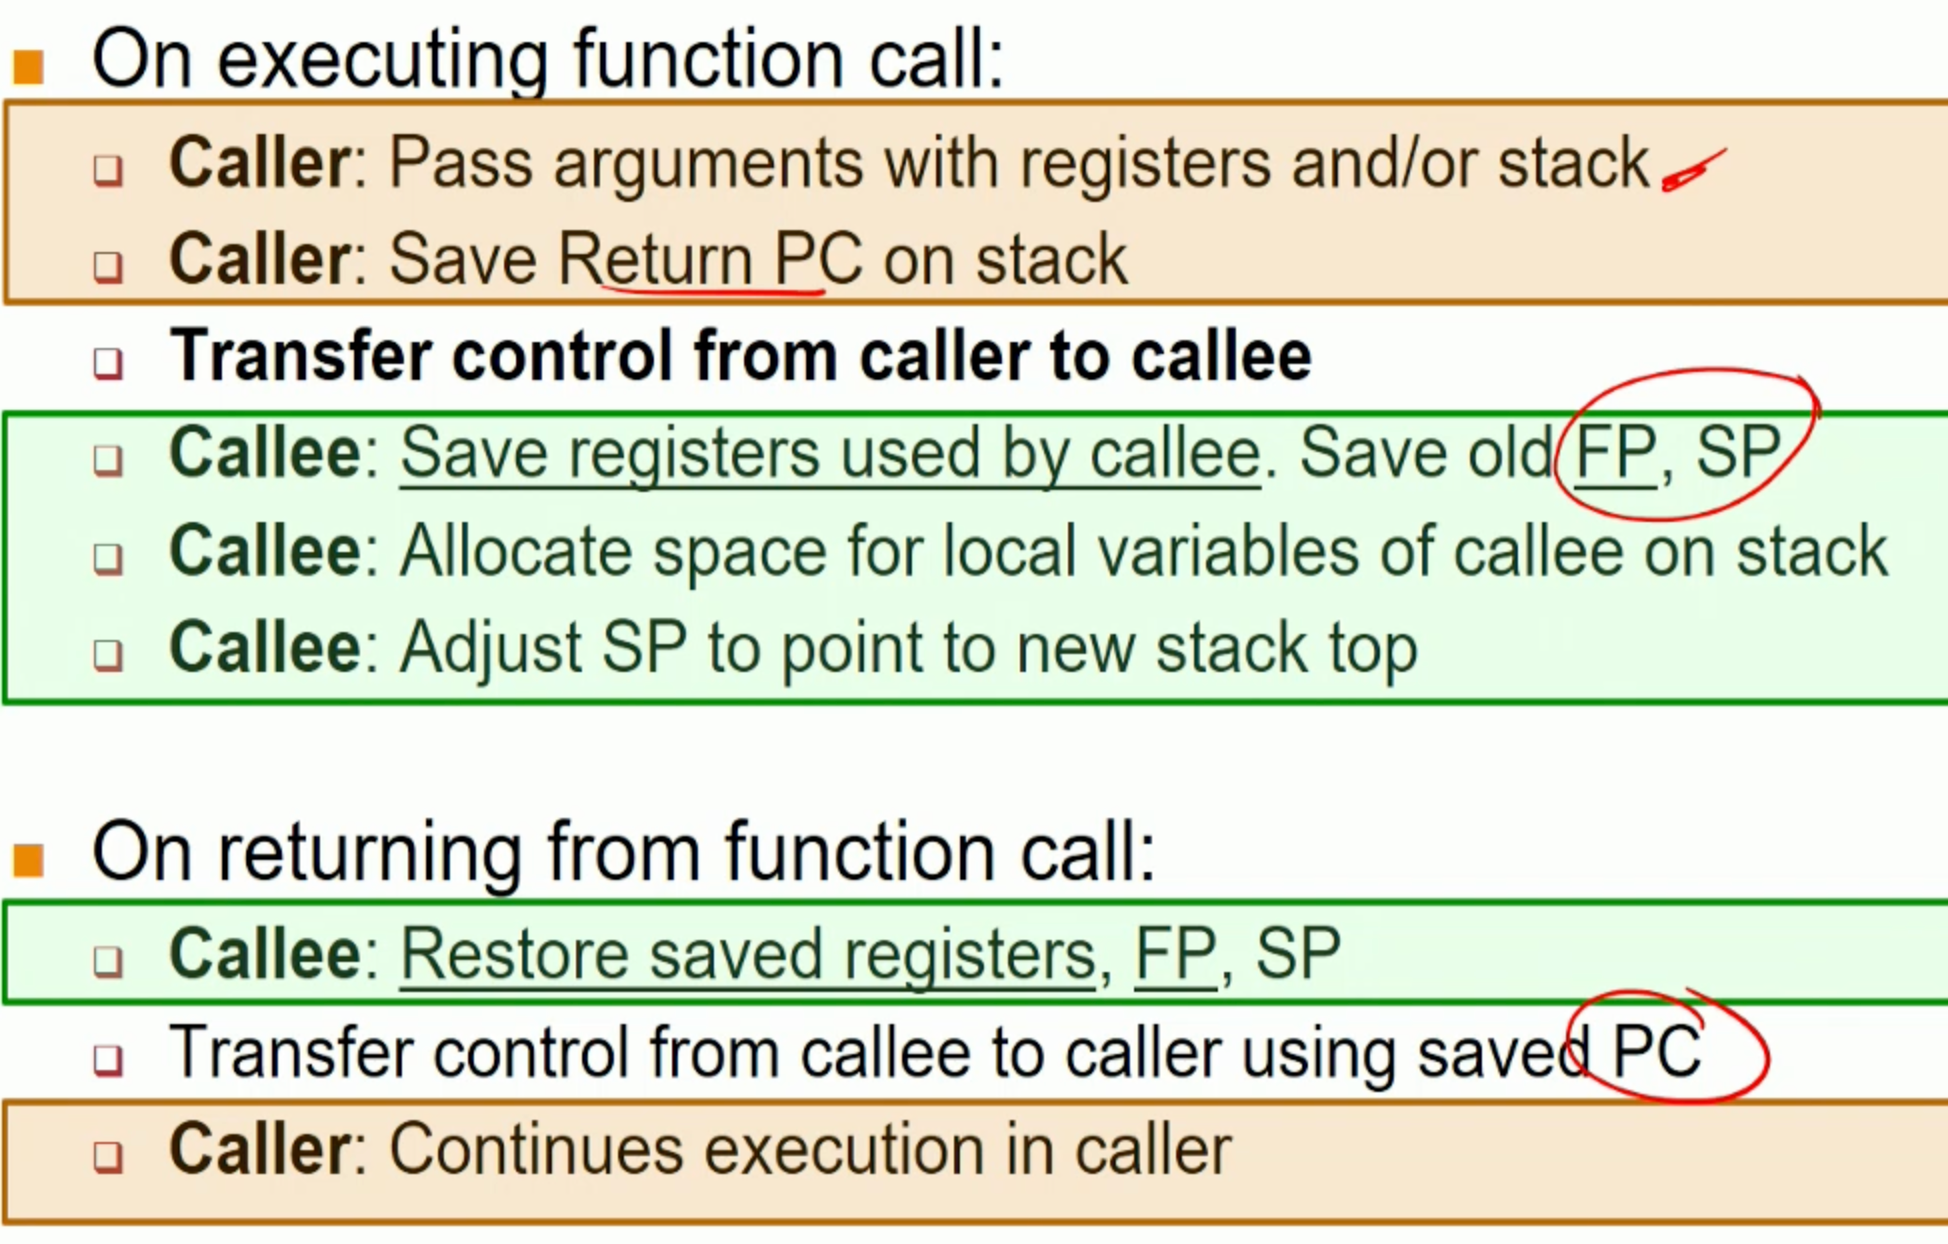
\includegraphics[scale=0.1]{stack-frame}\\
Information needed for function invocation - Stack frame
\begin{itemize}
	\item Return address of caller
	\item Arguments for the function
	\item Local variables
	\item Stack and frame pointer of caller
	\item GPR values (register spilling)
\end{itemize}
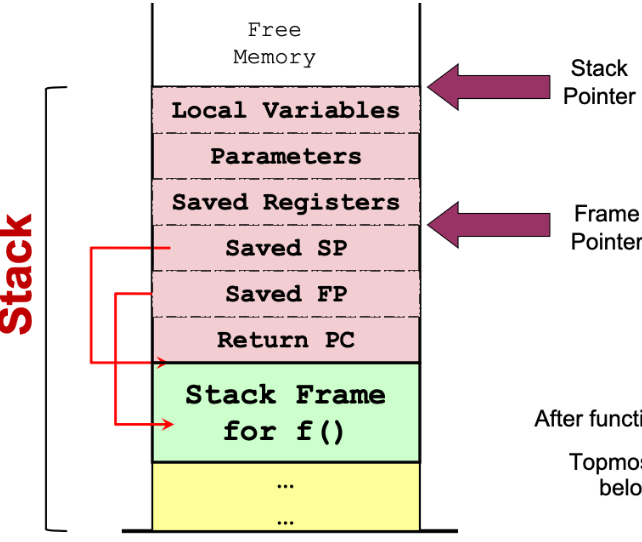
\includegraphics[scale=0.3]{stack-frame-diagram}\\
Callee stack frame will be on top of the caller


\subsection{Dynamic memory (Heap)}
Memory that the program/user specifies manually (eg. malloc, new)\\
Problems:
\begin{itemize}
	\item Allocated only at runtime
	\begin{itemize}
		\item Size not known at program compilation time
		\item Cannot specify a region in data 
	\end{itemize}
	\item No definite dellocation timing
	\begin{itemize}
		\item Must be freed explicitly by the program
		\item Cannot place in stack region
	\end{itemize}
\end{itemize}
Solution:\\
Add a region "Heap for dynamic allocation\\
Problems with heap memory:
\begin{itemize}
	\item Generation of holes in between data due to variable deallocation timing
\end{itemize}

%-----------------------------------------------------------------------------------------------------------------------
\subsection{OS context}
\subsubsection{Process identification}
Features:
\begin{itemize}
	\item Distinguish processes from each other (Unique)
	\item Communicated to the hardware
\end{itemize}
\subsubsection{Process state}
\begin{description}
	\item[New]{New process that may still be under initialization (not schedulable)}
	\item[Ready]
	\item[Running]{Executed on CPU}
	\item[Blocked]{Sleeping/waiting for event - cannot execute until event available}
	\item[Terminated]{Finished execution and requires OS cleanup}
\end{description}
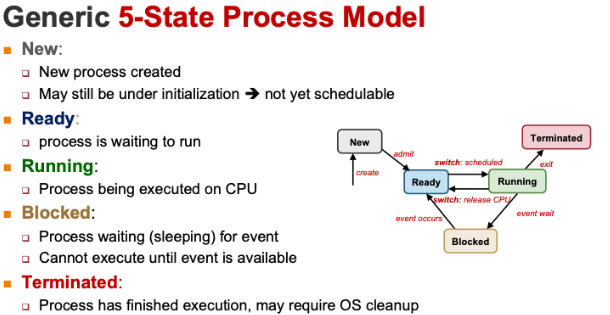
\includegraphics[scale=0.23]{process-model}
\subsection{Process control block}
Table representing all processes containing entire execution context stored in OS memory
\begin{itemize}
	\item PC, FP, SP and other GPR (only updated when swapped out)
	\item Memory region info (Text, data, heap and stack)
	\begin{itemize}
		\item It is a "point" to real memory space \textbf{NOT actual memory space used by process}
	\end{itemize}
	\item PID and process state
\end{itemize}
\subsubsection{Context switching}
\begin{enumerate}
	\item Interrupt or syscalls
	\item Save state of old process into PCB
	\item Reload state of new process from PCB
\end{enumerate}
\begin{itemize}
	\item Involves a change to kernel mode and back
\end{itemize}
\subsection{Exceptions and interrupts}
Exceptions
\begin{itemize}
	\item Synchronous (due to program execution)
	\item Machine level instructions arise errors
	\item Exception handler executed automatically in software (can be handled by programmer)
	\item Handled by OS which sends a signal to application to implement try-catch mechanism
\end{itemize}
Interrupts
\begin{itemize}
	\item Asynchronous (Can happen anytime)
	\item External events that cause execution to fail (hardware related errors)
	\item Program execution suspended and \textbf{interrupt handler} executed automatically
\end{itemize}
\subsubsection{Instruction execution}
\begin{enumerate}
	\item Read byte from PC and decode instruction
	\item Read 2 bytes to get the address/operands
	\item Perform ALU operations
	\item Store result into destination
	\item Check if any interruptions
\end{enumerate}
Interrupts can happen at anytime, and will remain pending until step 5 where it is handled

\subsubsection{Interruption handling}
\begin{enumerate}
	\item Push PC and status register into hardware
	\item Disable interrupts
	\item Read \keyword{Interrupt Vector Table}{Table where the OS stores address of all interrupt handlers}
	\item Switch to kernel mode
	\item Set PC to handler address and execute the instructions
\end{enumerate}
\begin{itemize}
	\item OS populates the IVT table with address of interrupt routines
	\item Hardware reads IVT to locate the handler
\end{itemize}
\subsection{System calls}
\keyword{Application Program Interface}{Provides way of calling facilities/services in kernel}\\
Synchronous function only done in kernel mode providing system services\\
Typically more expensive than library calls due to context switching\\
OS dependent anc cannot be avoided by any application
\subsubsection{Functions}
\begin{description}
	\item[Process control]{Direct processes like creating, terminating or synchronisation}
	\item[File/device manipulation]
	\item[Information maintenance]{Get system data, time, etc}
	\item[Communication]{Create, delete connections and send/receive messages}
\end{description}
\subsubsection{Method (Programming language specific)}
\begin{itemize}
	\item Library version with the same name and same arguments 
	\item User friendly library version
	\item Using func $long~syscall(long~number);$
\end{itemize}
\subsubsection{Mechanism}
\begin{enumerate}
	\item User invoke library call
	\item Place call number in the designated location
	\item Library call executes a special instruction (\textbf{TRAP/syscall}) to change user to kernel mode
	\item (in kernel) syscall handler is determined (by a \textbf{dispatcher})
	\item syscall handler is executed
	\item Syscall handler ends and control returned to the library call
	\item Return to user mode and continue normal function mechanism
\end{enumerate}


%--------------------------------------------------------------------------------------------------------------------
\section{03. Process abstraction in Unix}
Process information
\begin{description}
	\item[Pid]
	\item[Proc state]{Running, sleeping, stopped, zombie}
	\item[Parent pid]
	\item[Cumulative CPU time]{For scheduling}
\end{description}

\subsection{fork()}
Process creation
\begin{description}
	\item[Package]{unistd.h and sys/types.h}
	\item[return]{PID of newly created process(parent) and 0 (child process)}
\end{description}
\subsubsection{Behaviour}
\begin{itemize}
	\item Creates a child process
	\begin{itemize}
		\item \textbf{Copy} data of parent (Independent memory space)
		\item Unless explicitly modifying value at address, parent and child variables are distinct
		\item Sane code, same address space
		\item Differs by pid, ppid and fork() return value
	\end{itemize}
\end{itemize}

\subsubsection{Implementation}
Clone the parent process 
\begin{enumerate}
	\item Create address space of child process
	\item allocate new pid to child and pass to parent
	\item Create kernel process data structures
	\item Copy kernel environment of parent process
	\item Initialize child process context (pid, ppid, cpu\_time = 0)
	\item Copy memory regions from parent
	\begin{itemize}
		\item Very expensive operation
		\item Code, data, stack
	\end{itemize}
	\item Acquire shared resources
	\item Initialize hardware context for child process (copy parent registers)
\end{enumerate}

Problem: Memcopy is very expensive operation\\
Solution: Copy on write
\begin{itemize}
	\item Only duplicate a memory location when it is written to
\end{itemize}

\subsection{exec(@param)}
Replace current executing process image
\begin{itemize}
	\item Code and data replaced
	\item PID/PPID intact
	\item If fail, program just continues to run the next instruction
\end{itemize}
Format
\begin{description}
	\item[param]{char *path, char *arg0...}
	\begin{itemize}
		\item Note that last term MUST be \textbf{NULL} indicating end of argument list
	\end{itemize}
	\item[header]{unistd.h}
\end{description}

\subsection{exit(status)}
\begin{description}
	\item[return]{Does not return anything}
	\item[param]{int status - returned to the wait call}
\end{description}
\begin{itemize}
	\item Most system resource used by process are released on exit
	\item return from main() implicitly calls exit(0)
	\item Basic processes are not releasable
	\begin{itemize}
		\item Pid and status
		\item Process accounting info
	\end{itemize}
\end{itemize}

\subsection{wait(\&status)}
Parent child synchronisation
\begin{description}
	\item[param]{\&status - address to put return value}
	\item[header]{sys/types.h and sys/wait.h}
	\item[return]{pid of terminated process}
\end{description}
\begin{itemize}
	\item Call is blocking - suspend operation until at least one child terminates
	\item Cleans up remainder of child system resources (PID, status)
	\item waitpid - used for waiting for specific child process
\end{itemize}

\subsection{Orphan and zombie process}
\keyword{Zombie}{\textbf{All} processes that has exited but parent did not call wait}\\
\keyword{Orphan}{Child process whose parent has been terminated}
\begin{itemize}
	\item Parenthood will be propagated up to init which may use wait() to clean up
\end{itemize}


%--------------------------------------------------------------------------------------------------------------------
\section{04. Inter Process Communication}

\subsection{Mechanism}
\begin{itemize}
	\item Shared memory
	\item Message passing
	\begin{itemize}
		\item Pipes
		\item Signal
	\end{itemize}
\end{itemize}

\subsection{Shared memory}
Communication through read/write to shared memory\\
Advantages
\begin{description}
	\item[Efficient]{Only require OS to setup shared region once}
	\item[Ease of use]{Simple reads and write to memory}
	\begin{itemize}
		\item Implicit communication
		\item Can store any type of information
	\end{itemize}
\end{description}
Disadvantages
\begin{description}
	\item[Limited to single machines]{Less efficient over different system}
	\item[Need Sync]{Might have data races without synchronisation}
\end{description}
\keyword{Race condition}{System behaviour is dependent on the context/interleaving of process $\rightarrow$ unpredictable outcome}
\subsubsection{Steps}
\begin{enumerate}
	\item Create/locate a shared memory region M
	\item Attach M to process memory space
	\item Read from/write to M
	\item Detach M from memory space after use
	\item Destroy M
	\begin{itemize}
		\item Only one process need to do this
		\item Can only destroy if M is not attached to any process
	\end{itemize}
\end{enumerate}

\subsection{Message Passing}
Explicit communication through exchange of message
\begin{description}
	\item[Naming]{Have to identify the parties in the communication}
	\item[Synchronisation]{Behaviour of sending/receiving operations}
\end{description}
\begin{itemize}
	\item Messages have to be stored in kernel memory space
	\item All sending/receiving operations have to be done through syscalls
\end{itemize}
\subsubsection{Direct communication}
Sender/receiver explicitly name parties in communication
\begin{itemize}
	\item One link per pair of communicating processes
	\item Need to know identity of other party
\end{itemize}

\subsubsection{Indirect communication}
Message storage (\textbf{Mailbox/Port})
\begin{itemize}
	\item Can be shared among a number of processes
\end{itemize}

\subsubsection{Synchronisation behaviour}
Blocking
\begin{itemize}
	\item send and receive is blocked until a message has received/sent (other party is ready)
\end{itemize}
Non-blocking (asynchronous)
\begin{itemize}
	\item execute immediately and sends information to somebody OR returns empty handed
\end{itemize}
Typically, receive is synchronous and send is asynchronous\\
BUT send just buffers the message and only sends the message when the receiver is receiving (no loss)\\
Message buffers
\begin{itemize}
	\item Under OS control 
	\item Decouples sender and receiver -\> less sensitive to variation in execution
	\item Mailbox capacity declaration in advance
\end{itemize}
\textbf{Rendezvous}
\begin{itemize}
	\item Synchronous message passing 
	\item Sender is blocked until receiver sends matching receive
	\item No buffering needed
\end{itemize}

\subsubsection{Pros}
\begin{itemize}
	\item Applicable beyond a single machine
	\item \keyword{Portable}{Easily implemented on many platforms and processing environments}
	\item Easier synchronisation
	\begin{itemize}
		\item Implicit via send/receive behaviour
		\item Communication and synchronisation is done simultaneously
	\end{itemize}
\end{itemize}
\subsubsection{Cons}
\begin{description}
	\item[Inefficient]{Usually requires OS intervention every operation}
	\item[Difficult to use]{Requires information packing into specific format}
\end{description}

\subsection{Unix Pipes}
3 different communication channels to user
\begin{enumerate}
	\item stdin - standard in bounded to keyboard input
	\item stderr - used for error messages
	\item stdout - linked to screen
\end{enumerate}
$"|"$ symbol for linking input/output channels of each process to each other\\
Create communication channel with 2 ends (one reading, one writing)
\begin{itemize}
	\item Producer-consumer relationship
	\item Like anonymous file reading information FIFO
\end{itemize}
\subsubsection{Synchronisation}
\begin{itemize}
	\item Circular bounded byte buffer with implicit synchronization
	\item Writer wait when buffer is full
	\item Reader wait when buffer is empty
	\item Unidirectional (one write one read exclusively) vs bidirectional (any end for reading and writing)
\end{itemize}
\subsubsection{pipe(@param)}
\begin{description}
	\item[param]{array of file descriptors}
	\item[return]{0 for success, != for errors}
\end{description}
\subsection{Unix signals}
Asynchronous notification about an event sent to process/threads
\begin{itemize}
	\item Handle signal via default or user defined/supplied handlers(not all signals)
	\item Can only call async safe functions within handler (signal/wait cannot be called in POSIX)
	\item eg. Kill, stop, continue, error
\end{itemize}
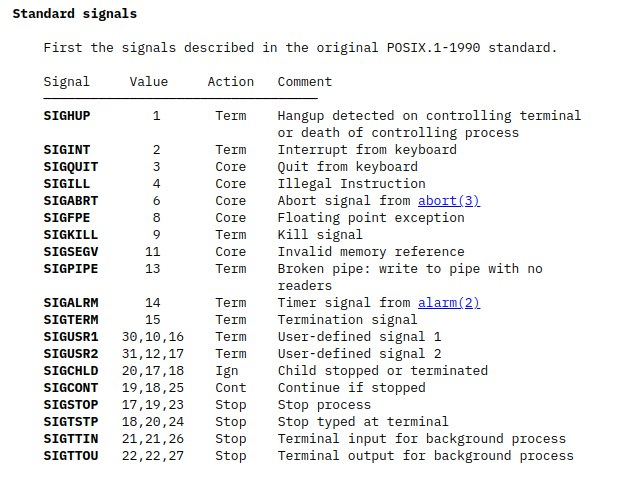
\includegraphics[scale=0.35]{common-signals}

%--------------------------------------------------------------------------------------------------------------------

\section{05.Process scheduling}
Concurrency
\begin{itemize}
	\item Multiple process progress at the same time
	\item Virtual parallelism (threading, context switching)
	\item Physical parallelism (multicore, multi CPU)
\end{itemize}

\subsection{Scheduling}
More ready processes vs limited CPU
\begin{itemize}
	\item Each process diff CPU usage
	\item \keyword{Scheduling algorithms}{Deciding the process to run based on environment and process behaviour}
	\item Processes have phases of io-bound and cpu intensive activities
\end{itemize}
Processing environment (sorted by increasing user interaction and response times):
\begin{enumerate}
	\item Batch
	\item Interactive
	\item Real time
\end{enumerate}
\subsection{Objectives}
\begin{description}
	\item[Fairness]{Should get fair share of CPU time n prevent \keyword{starvation}{processes never have access to CPU}}
	\item[Utilization]{Hardware is used all the time}
\end{description}
\keyword{non-preemptive}{Process gives up resources voluntarily}
\keyword{preemptive}{Process given a fixed quota to run and is suspended for other processes}
\subsection{Timeline}
\begin{enumerate}
	\item Scheduler is triggered (OS take over)
	\item Context switching can happen and current process information stored and placed back in queue
	\item Pick process to run using algorithm and setup its context
\end{enumerate}

\subsection{Batch}
Non-preemptive used dominantly cos minimal user interaction needed
\subsubsection{Objectives} 
\begin{description}
	\item[Turnaround time]{Total time till finish running \textbf{including waiting} (finish time - arrival time)}
	\item[Throughput]{Rate of task completion}
	\item[Makespan]{Total time to complete \textbf{ALL} tasks}
	\item[CPU utilization]{Percentage of \textbf{time} CPU is used}
\end{description}
\subsubsection{Algorithms}
\begin{enumerate}
	\item First Come First Serve (FCFS)
	\begin{itemize}
		\item Scheduled using FIFO queue based on arrival time (bad turnaround time)
		\item Guarantee no starvation - number of tasks in front of task is strictly decreasing
		\item Reordering can reduce waiting time 
		\item \keyword{Convoy Effect}{Not all hardware resources are used concurrently because a process blocks it}
	\end{itemize}
	\item Shortest Job First (SJF)
	\begin{itemize}
		\item Choose tasks with smallest total CPU time
		\item Estimate CPU time for tasks in advance using the previous CPU-bound phases
		\item $Estimated_{n+1} = \alpha Actual_{n} + (1-\alpha) Predicted_{n}$
		\item Starvation is possible as long tasks end up continuously waiting
	\end{itemize}
	\item Shortest Remaining Time (SRT)
\end{enumerate}

\subsection{Interactive system}
\subsubsection{Objectives}
\begin{description}
	\item[Response time]{Time between request and response by system}
	\item[Predictability]{Decreased variation in response time}
	\item[Premptive scheduling]
\end{description}
\begin{itemize}
	\item Periodic scheduler with time interrupts
	\item \keyword{Time quantum}{Execution duration given to a process}
	\begin{itemize}
		\item Constant(regardless whether the process has given up processing halfway) OR Variable(full time quantum given to a process)
	\end{itemize}
\end{itemize}

\end{multicols*}
\begin{multicols*}{3}
\subsubsection{Algorithms}
\begin{enumerate}
	\item Round Robin (RR)
	\begin{itemize}
		\item Store tasks in FIFO queue and pick tasks to run until
		\begin{enumerate}
			\item Fixed time slice elapsed
			\item Task gives up CPU voluntarily
			\item Task blocks
		\end{enumerate}
		\item Task placed at end of queue to wait for next turn
		\item Response time guaranteed bounded by num task \* time quantum
		\item Timer interrupt needed
		\item Choice of time quantum duration is important 
		\begin{itemize}
			\item Longer quantum: Better utilization but greater wait time
			\item Shorter quantum: Bigger overhead/ lower utilization but shorter wait time
		\end{itemize}
		\item Poor performance when there are many jobs all exceeding time quantum -\> high overhead from context switching
	\end{itemize}
	\item Priority scheduling
	\begin{itemize}
		\item Assign tasks processes priorities based on impt and select them
		\item Starvation for low priority tasks
		\begin{itemize}
			\item Solution: 
			\item Lower priority every time the process have executed
			\item Give processes a time quantum
		\end{itemize}
		\item \keyword{Priority Inversion}{Lower priority tasks locks the resources used by a higher priority task leading to deadlock OR allowing lower priority tasks to run before}
		\begin{itemize}
			\item Solution:
			\item Temporarily increase priority of tasks that lock resources until it unlocks
			\item Low priority task inherit the priority of high priority tasks which is restored once unlocked
		\end{itemize}
	\end{itemize}
	\item Multi-level Feedback Queue (MLFQ)
	\begin{itemize}
		\item Runs processes with higher priorities but lower priority when the job fully utilise its time quantum
		\item Processes that voluntarily gives up/blocks before time quantum retains its priority
		\item New processes have highest priority
		\item Processes with same priority run in RR
		\item Long CPU processes are starved as its priority becomes very low and cannot complete
		\begin{itemize}
			\item Solution: Occassionally reset tasks to full priority 
		\end{itemize}
		\item Processes can exploit and voluntarily give up to retain its priority
		\begin{itemize}
			\item Solution: Peg priority based on total CPU usage instead 
		\end{itemize}
	\end{itemize}
	\item Lottery scheduling
	\begin{itemize}
		\item Give out tickets to processes for various system resources and randomly pick winners to be granted the resources
		\item \keyword{Responsive}{Newly created processes can immediately join the lottery}
		\item Good control - Process can be assigned quantity of tickets and resources which can be shared among its children/threads
		\item Simple implementation
	\end{itemize}
\end{enumerate}
%--------------------------------------------------------------------------------------------------------------------
\section{06.Synchronisation primitives}
\subsection{Race condition}
\begin{itemize}
	\item Execution of sequential processes should be \keyword{deterministic}{Repeated execution returns the same result}... however,
	\item Process sharing modifiable resources AND execute concurrently by interleaving may cause synchronization problems -\> non deterministic outcomes
	\item Order determines the execution outcome
\end{itemize}

\subsection{Critical section}
Region where unsynchronised access could lead to incorrectly interleaving scenarios\\
Only \textbf{ONE} process should be in the critical section at one time
\subsubsection{Properties}
\begin{description}
	\item[Mutual exclusion/Mutex]{All other processes should be blocked from entering critical section if occupied}
	\item[Progress]{If no process occupying section, waiting process should be granted access}
	\item[Bounded wait]{Upper bound on number of times other processes can enter critical section before a waiting process}
	\item[Independence]{Process not in critical section should not block other process}
\end{description}
\subsubsection{Incorrect synchronization}
\begin{description}
	\item[Deadlock]{All processes blocked}
	\item[Livelock]{Processes keep changing states to avoid deadlock resulting in no progress (Deadlock avoidance mechanism)}
	\item[Starvation]
\end{description}
\subsection{Implementations}
\begin{itemize}
	\item High level language implementation (Peterson Algorithm)
	\begin{itemize}
		\item Busy waiting - Repeatedly tests while-loop condition instead of going into blocked state (Wastes CPU power)
		\item Low level - Error prone and complicated
		\item Not general - cannot extend to allowing multiple access instead of Mutex
	\end{itemize}
\end{itemize}
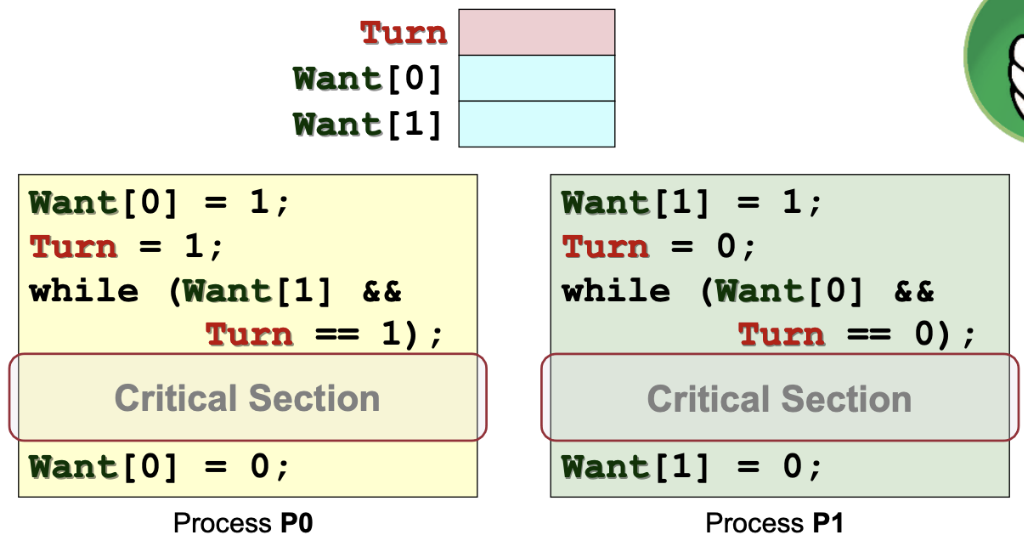
\includegraphics[scale=0.46]{peterson-algorithm}
\begin{itemize}
	\item Assembly implementation
	\begin{itemize}
		\item Atomic instruction to load value and replace value in memory location (\textbf{TestAndSet})
		\item \keyword{Atomicity}{Prevents race condition of process viewing and upon modification, the value changes}
		\item No bounded wait unless fair scheduling algorithm employed
		\item Employs busy waiting still
	\end{itemize}
\end{itemize}
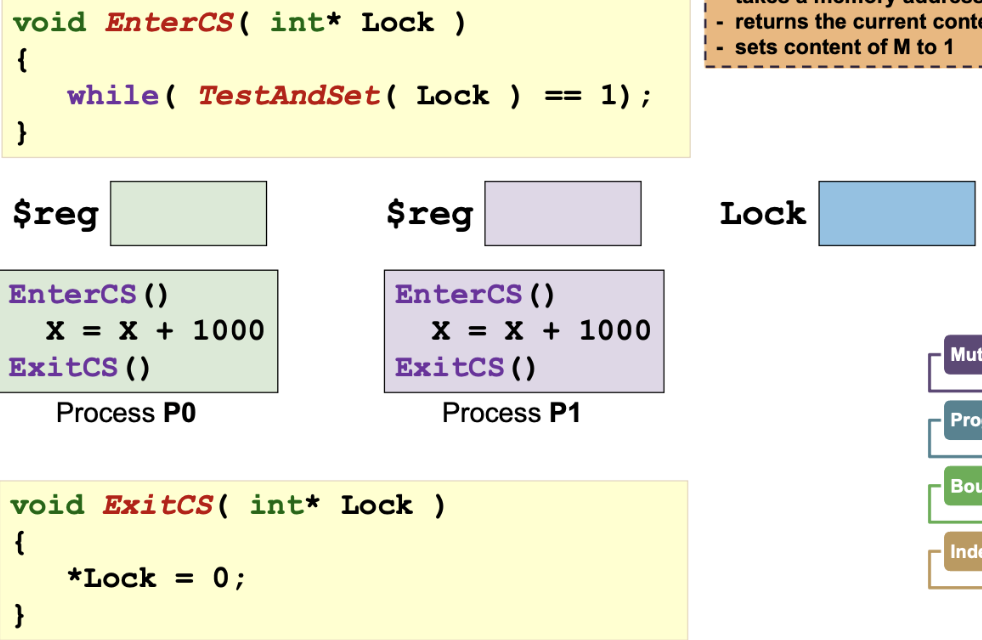
\includegraphics[scale=0.5]{test-and-set}
\begin{itemize}
	\item High level synchronization mechanism (Semaphore)
	\begin{itemize}
		\item Generalised mechanism to block a number of processes (sleeping), $S$, and unblock sleeping processes
		\item \keyword{wait()}{Blocks if $S\leq 0$, decrement S}
		\item \keyword{signal()}{Increment $S$, wake up sleeping processes, operation \textbf{never} blocks}
		\item \keyword{Invariant}{$S_{current} = S_{initial} + N_{signal} - N_{wait}$}
	\end{itemize}
\end{itemize}
\subsubsection{Conditional variables}
\begin{itemize}
	\item Tasks wait for certain events to happen
	\item Event completion/begin is broadcasted
\end{itemize}
\subsubsection{POSIX semaphore}
\begin{description}
	\item[header]{semaphore.h}
	\item[wait]{pthread\_mutex\_unlock}
	\item[signal]{pthread\_mutex\_lock}
\end{description}

%--------------------------------------------------------------------------------------------------------------------
\section{Midterm}
\begin{itemize}
	\item \keyword{Tail-call optimization}{Stack frame can be replaced in iterative recursion since all information is retained in the 'return' function call at every iteration}
\end{itemize}

%--------------------------------------------------------------------------------------------------------------------
\section{07.Threads}
\subsection{Motivation}
\begin{itemize}
	\item Processes are expensive
	\begin{itemize}
		\item Process creation via fork() duplicates memory space and process context
		\item Requires context switching and saving/restoring process information repeatedly
	\end{itemize}
	\item Hard to communicate with each other
	\begin{itemize}
		\item Independent memory space (IPC communication only)
	\end{itemize}
	\item Need easy way to execute some instructions simultaneously (more threads of control to same process)
\end{itemize}
\subsection{Features}
\begin{itemize}
	\item \keyword{Multithreaded process}{Single process with multiple threads}
	\item Threads share the same \textbf{Memory context}(Text, data, heap) and \textbf{OS context}(PID)
	\item Contains unique information
	\begin{itemize}
		\item Identification (thread id)
		\item Registers (GPR and special)
		\item Stack
	\end{itemize}
\end{itemize}

\subsection{Benefits}
\begin{description}
	\item[Economy]{Less resources to manage}
	\item[Resource sharing]
	\item[Responsiveness]
	\item[Scalability]{Can take advantage of multiple CPUs}	
\end{description}

\subsection{Problems}
\begin{itemize}
	\item Syscall concurrency
	\begin{itemize}
		\item Parallel execution of threads may result in parallel syscalls
	\end{itemize}
	\item Process behaviour
	\begin{itemize}
		\item Unable to impact process operations
	\end{itemize}
\end{itemize}

\subsection{Thread implementation}
\begin{enumerate}
	\item User thread
	\begin{itemize}
		\item Implemented as a user library -\> More flexible and configurable
		\item Runs on any OS
		\item Kernel unaware of threads in process (scheduling at process level)
		\item If process is blocked, all the threads in the process cannot run 
	\end{itemize}
	\item Kernel thread
	\begin{itemize}
		\item Implemented in the OS through syscalls (slower and more resource intensive)
		\item Scheduling among threads instead of via process
		\item Use threads in kernel operations
		\item Less flexible
		\begin{itemize}
			\item Used by all multithreaded programs so kernel must cater to all
			\item Balance btw many and less features
		\end{itemize}
	\end{itemize}
	\item Hybrid thread
	\begin{itemize}
		\item OS schedules on kernel threads
		\item User threads can be bound to kernel threads
		\item If the user thread is blocked, the kernel thread that it is assigned to is blocked and the OS will execute another kernel thread
		\item Lead to greater flexibility
	\end{itemize}
\end{enumerate}

\subsection{Posix Threads (pthreads)}
\subsubsection{pthread\_create}
\begin{description}
	\item[param]{tid, attributes, \&function, function\_params}
	\item[return]{0 success, != 0 fail}
\end{description}

\subsubsection{pthread\_exit}
\begin{description}
	\item Automatically called after function finishes
	\item[param]{exit\_value}
	\item[behaviour]{return value of function will be the "exit value"}
\end{description}

\subsubsection{pthread\_join}
\begin{description}
	\item[param]{tid, \keyword{\&status}Exit value returned by target pthread}
\end{description}

%--------------------------------------------------------------------------------------------------------------------
\section{08. Classic synchronisation problems}
Use cases of synchronisation (mutexes)

\subsection{Producer Consumer}
\begin{itemize}
	\item Processes share a bounded biffer of size K
	\begin{itemize}
		\item Producers produce items to insert in buffer when not full
		\item Consumers remove items from buffer when non-empty
	\end{itemize}
	\item Busy waiting vs blocking version and message passing
\end{itemize}
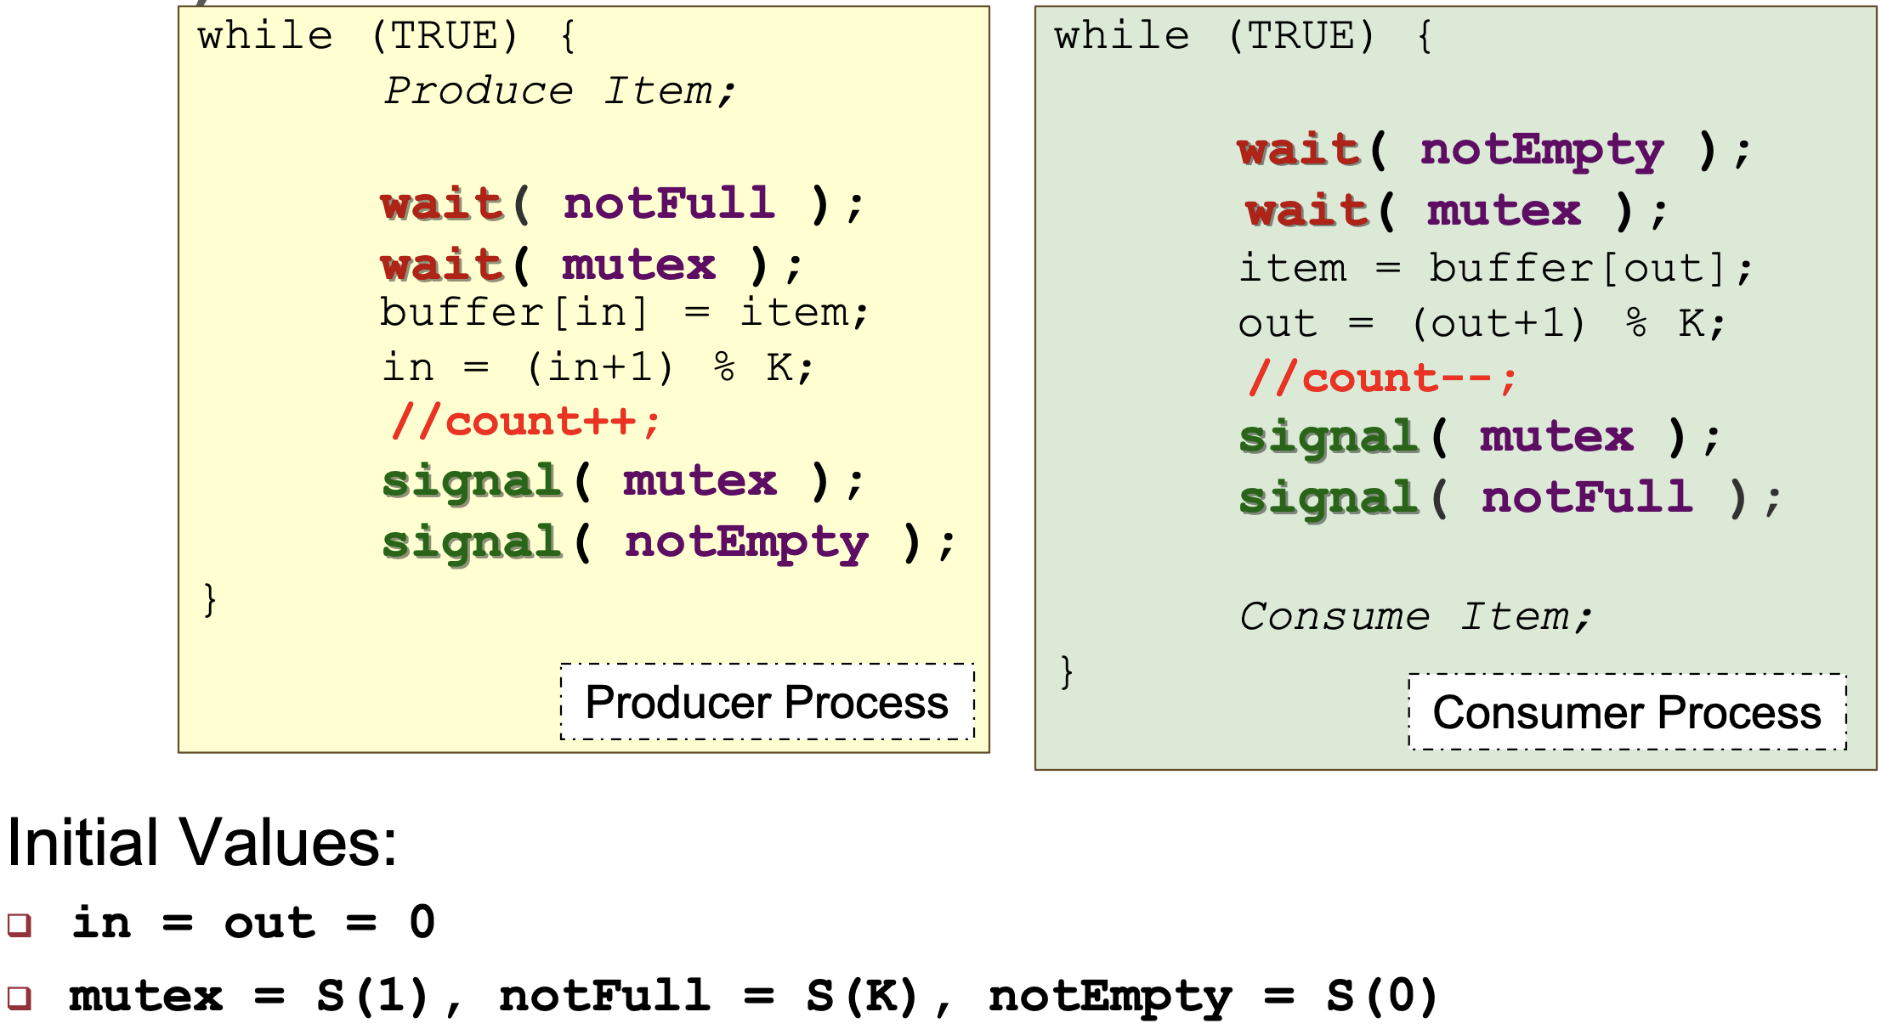
\includegraphics[scale=0.28]{producer-consumer}

\subsection{Reader writer}
\begin{itemize}
	\item Processes share data structure D
	\begin{itemize}
		\item Reader retrieves information from D (multiple concurrent accesses)
		\item Writer modifies information from D exclusively
	\end{itemize}
	\item Starvation of the writer as readers can continue to occupy the resource continuously
\end{itemize}
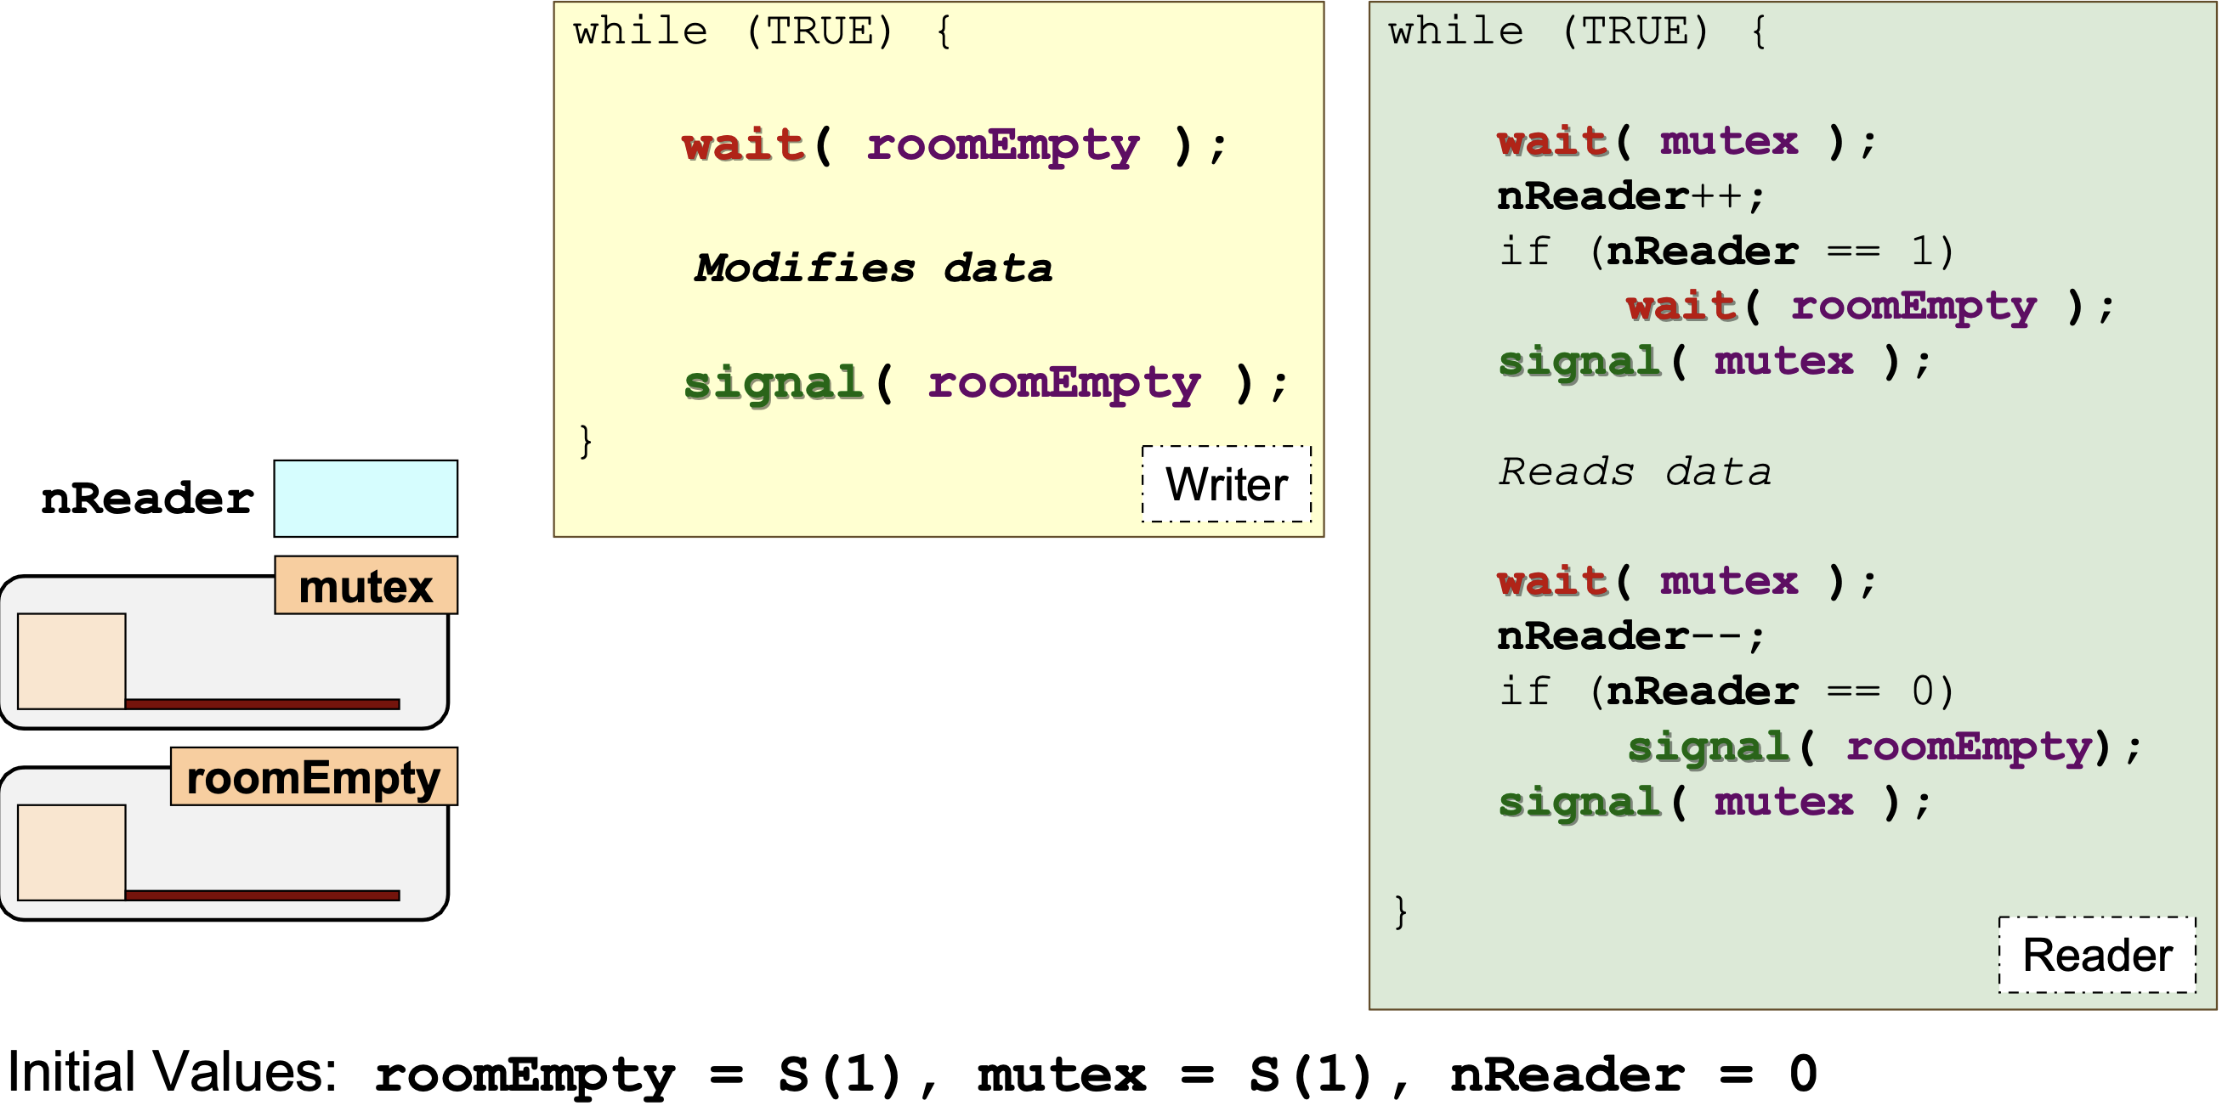
\includegraphics[scale=0.24]{reader-writer}

\subsection{Dining philosophers}

\includegraphics[scale=0.2]{dining-philosophers-spec}
\begin{itemize}
	\item Single chopsticks between philosophers sitting around a table
	\item Philosophers need pair to eat without deadlocks and starvation
	\item Philosophers makes the same decision (takes the same side of chopsticks everytime)
\end{itemize}
\subsubsection{Livelock}
\begin{itemize}
	\item To prevent deadlock, philosophers put down chopstick if cannot get the other side
	\item Livelock because all philosophers take chopstick, put down ....
\end{itemize}

\subsubsection{Limited eater}
\begin{itemize}
	\item One of the philosophers delay their eating temporarily until either side finishes
	\item All philosophers can complete their execution pigeonhole theorum (more chopsticks than philos)
	\item Not fair to the philosopher not eating (How to decide who stops operation?)
\end{itemize}

\subsubsection{Tanenbaum Solution}
\begin{itemize}
	\item Randomly decide which side chopstick the philosophers take first
\end{itemize}

%------------------------------------------------------------------------------------------------------------------------------

\section{09. Memory abstraction}
\subsection{Basics}
\subsubsection{Hardware}
\begin{itemize}
	\item uses Random Access Memory
	\begin{itemize}
		\item Access latency approximately constant regardless of location
	\end{itemize}
	\item Can be treated as a 1D array of \keyword{AU}{Addressable unit}
	\item \keyword{Contiguous}{Consecutive memory address with unique index (physical address)}
\end{itemize}
\subsubsection{Memory usage of process}
Types of data
\begin{enumerate}
	\item \keyword{Transient data}{Valid only for a specific duration}
	\item \keyword{Persistent data}{Valid for complete duration of prgm until explicitly deallocated}
\end{enumerate}
\subsubsection{Role of OS}
\begin{enumerate}
	\item Allocate, manage and protect memory space for each process
	\item Provide memory-related system calls to processes
	\item Manage memory space for internal OS use
\end{enumerate}

\subsection{Memory abstractions}
\subsubsection{Motivation}
\begin{itemize}
	\item Processes assume memory starts at 0 and occupy the same memory location
	\item Difficult to protect memory space
\end{itemize}
\subsubsection{Solutions (?)}
\begin{itemize}
	\item Address reallocation
	\begin{itemize}
		\item Change all the memory addresses when starting process to the new changed memory address
		\item Problems: Slow runtime because have to run through all the instructions
	\end{itemize}
	\item Base and limit registers
	\begin{itemize}
		\item Base register as the "starting point" of all memory references
		\item Limit register as the range of memory space of current process (protect memory space integrity)
		\item All memory references are compiled as an offset of base register 		
	\end{itemize}
\end{itemize}
\subsubsection{Logical address}
\begin{itemize}
	\item How the program views its memory space
	\item Mapping between physical and logical address needed
	\item Self contained, independent logical memory space
\end{itemize}
\subsection{Contiguous Memory allocation}
Same process occupies memory as one piece during whole execution
\subsubsection{Fixed size partitions}
\begin{itemize}
	\item Fixed number of partitions and size (Minimum addressable units of partition is larger)
	\item \keyword{Internal fragmentation} Wasted leftover space when process does not occupy whole partition
	\item Pros: Easy to manage and fast to allocate
	\item Cons: Partition size need to be large enough to contain the largest process without wasting space
\end{itemize}
\subsection{Variable size partitions}
\keyword{External fragmentation}{Waste of space outside of partition (unallocated to any process)}
\begin{itemize}
	\item Pros: Flexible and removes internal fragmentation
	\item Cons: Need more info in OS and takes longer time to locate appropriate region
\end{itemize}
\subsubsection{Allocation algorithms}
\begin{itemize}
	\item First fit 
	\begin{itemize}
		\item Take the first hole large enough
		\item Fastest runtime (don't have to iterate through all the free partitions)
		\item May be inefficient (high external fragmentation)
	\end{itemize}
	\item Best fit
	\begin{itemize}
		\item Choose the smallest partition that fits the information
		\item Slower runtime but more efficient
	\end{itemize}
	\item Worst fit
	\begin{itemize}
		\item Choose the largest partition 
		\item Try to ensure that there is enough free space in the large partition for other process
	\end{itemize}
\end{itemize}
\subsubsection{Merging and Compaction}
Merging
\begin{itemize}
	\item When occupied partition is freed, it can join surrounding partitions to form a larger partition
\end{itemize}
Compaction
\begin{itemize}
	\item Mving occupied partitions around to create bigger consolidated holes
\end{itemize}

\subsubsection{Multiple free lists}
\begin{itemize}
	\item Keep multiple lists of different hole sizes and take the hole from list that most closely match request size
	\item Partition size increases exponentially but fast allocation (compared to iterating through all address to find free partitions)
\end{itemize}
\textbf{Buddy system}
\begin{itemize}
	\item Free block split into half repeatedly to meet request size
	\item Merge buddy blocks when both free
	\item Pros: Efficient partition splitting, deallocation and for locating good match
\end{itemize}
Allocation algorithm ($2^k$ is largest allocatable block)
\begin{enumerate}
	\item Find smallest s such that $2^s \geq N$
	\item Access A[S] for free block
	\begin{enumerate}
		\item Free block exists
		\begin{itemize}
			\item Remove block from free block list and allocate
		\end{itemize}
		\item Find smallest R from S+1 - K such that A[R] has a free block B
		\item Split B and restart from step 1
	\end{enumerate}
\end{enumerate}
Deallocation algorithm
\begin{enumerate}
	\item Check if buddy is free
	\begin{enumerate}
		\item If buddy is free remove both blocks from list and merge to get a larger block
	\end{enumerate}
	\item If buddy not free then insert block into list
\end{enumerate}
2 blocks B and C of size $2^S$ are buddies if
\begin{itemize}
	\item Lowest S bits (0..S-1) of B and C are identical
	\item S+1th bit of B and C is different
\end{itemize}

\section{10. Disjoint memory schemes}
\begin{itemize}
	\item Processes informations can be split into disjoint physical memory chunks
\end{itemize}
\subsection{Paging scheme}
\begin{itemize}
	\item Divide into \keyword{physical frames}{memory split into regions of fixed size}
	\item Frames sizes are decided by hardware
	\begin{itemize}
		\item Reduce number of access to memory
		\item Dedicated component to support paging by speeding address translation
	\end{itemize}
	\item Logical memory also split into same size (logical page)
\end{itemize}
\subsubsection{Page table}
\begin{itemize}
	\item Lookup mechanism for mapping logical pages to physical frames
	\item Physical address = $frame_number*sizeof(physical_frame)+offset$
	\item Note that frame sizes should be a power of 2 (ease of calculation)
	\item No external fragmentation - any information can be stored in any page
	\item Possible internal fragmentation (but low)
	\item Abstraction of logical and physical address
	\begin{itemize}
		\item Greater flexibility
	\end{itemize}
\end{itemize}
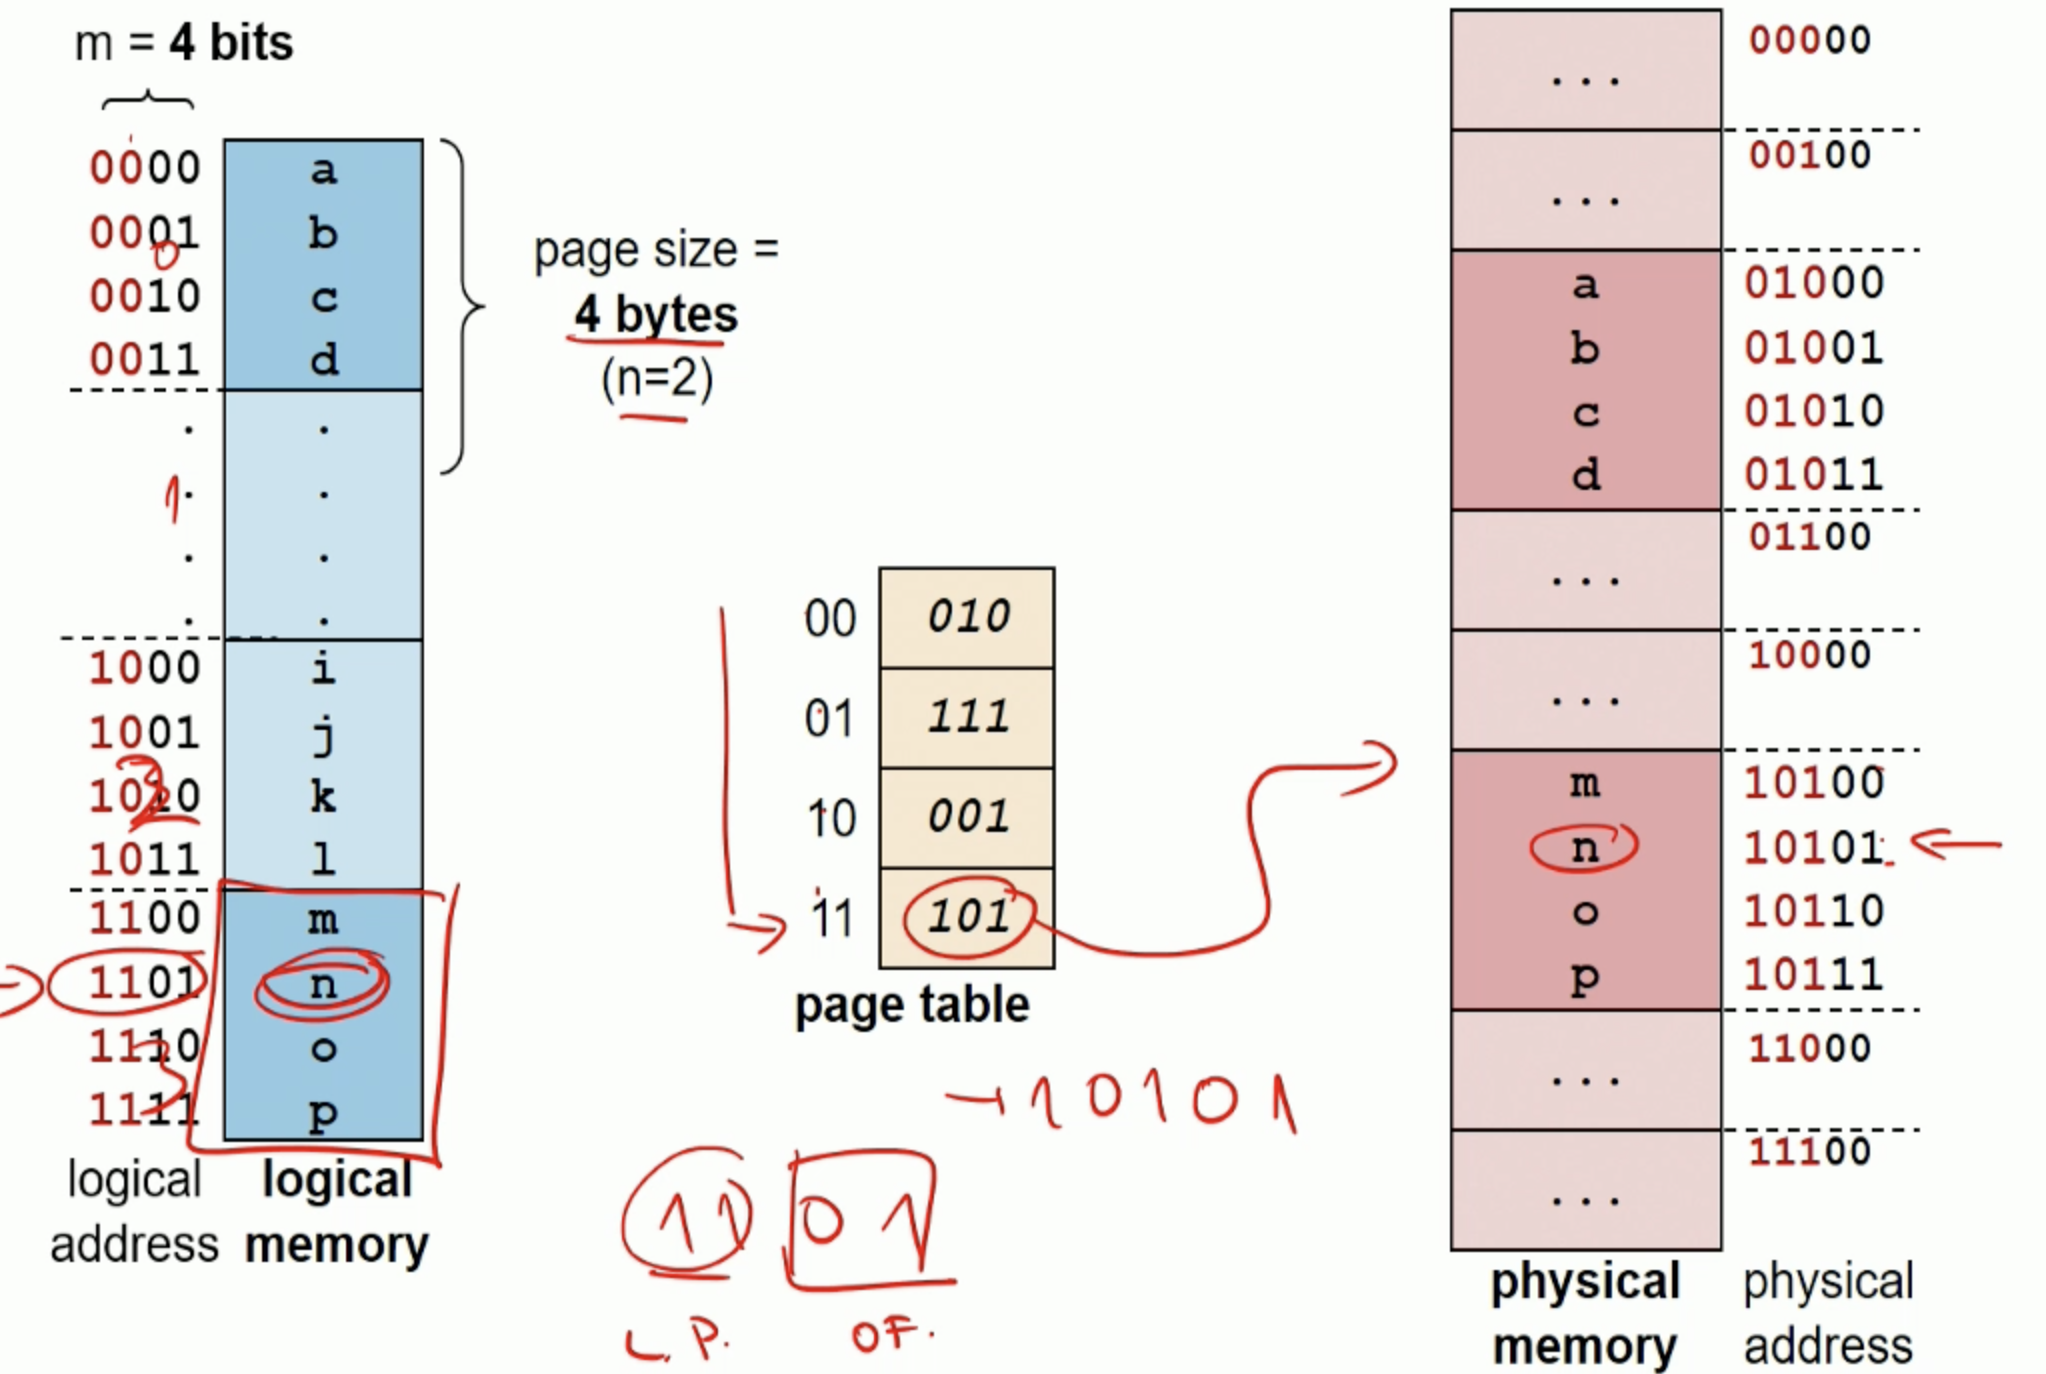
\includegraphics[scale=0.2]{paging-example}
\subsubsection{Implementation}
\begin{enumerate}
	\item Pure software
	\begin{itemize}
		\item OS stores page table information in PCB with 2 access to memory per reference
		\begin{enumerate}
			\item Read the indexed page table entry to get the frame number
			\item Access the actual memory item
		\end{enumerate}
	\item Memory context of each process includes page table/pointers to page table
	\end{itemize}
	\item Hardware support
	\begin{itemize}
		\item Contain \keyword{Translation Look-aside Buffer}{Specialized on-chip component to cache page table entries}
		\item Use page numbers to search TLB associatively
		\item Possible to have multiple TLB per core
		\begin{description}
			\item[TLB-hit]{Frame number retrieved to generate physical address}
			\item[TLB-miss]{Memory access to page table -\> retrieved frame number used to generate physical address and update TLB}
		\end{description}
		\item Very small and fast (reducing average Memory Access Time)
		\begin{itemize}
			\item $P(TLB~hit)*latency(TLB~hit)+P(TLB~miss)*latency(TLB~miss)$
			\item Latency of filling in TLB hidden by hardware
		\end{itemize}
		\item Part of hardware context, so entries will be flushed when context switch occurs
		\begin{itemize}
			\item Save pointer to prev process' page table in PCB 
			\item Ensure process does not get incorrect translation
		\end{itemize}
	\end{itemize}
\end{enumerate}

\subsubsection{Paging scheme}
\begin{itemize}
	\item Access-right bits
	\begin{itemize}
		\item Enforce protection like read, write execute permissions
		\item Memory access checked against access-right bits in hardware
	\end{itemize}
	\item Valid Bit
	\begin{itemize}
		\item Exclude pages that are out-of-range for particular process from mapping
		\item Check against bits in hardware whether the page can be accessed by process
	\end{itemize}
	\item Page sharing
	\begin{itemize}
		\item Allow several processes to share the same physical memory frame
		\item Shared code pages (code that may be used by many processes)
		\item Copy on write (share pages until one tries to change value from it)
	\end{itemize}
\end{itemize}

\subsection{Segmentation scheme}
\subsubsection{Motivation}
\begin{itemize}
	\item Process contains different types of memory regions (data, text, heap, stack)
	\begin{itemize}
		\item Does not really matter the order of memory regions
	\end{itemize}
	\item Regions are variable sized and grow/shrink at execution time 
	\begin{itemize}
		\item Provision gaps in-between
		\item Difficult to check what is the permissions of memory access (which range it is)
	\end{itemize}
\end{itemize}
\subsubsection{Implementation}
\begin{itemize}
	\item Process broken into segments of variable sizes
	\item Manage memory at level of memory segments
	\item Mapped into contiguous physical partitions of the same size
	\begin{itemize}
		\item Contains name (base address + segment\_id) and limit (range of segment)
		\item 
	\end{itemize}
\end{itemize}
\subsubsection{Evaluation}
\begin{itemize}
	\item + Independent contiguous memory space matches programmers view of memory
	\item + More efficient bookkeeping
	\item + Segments can grow/shrink and be protected/shared independently
	\item - Cause external fragmentation due to variable sized contiguous memory regions
\end{itemize}
\subsection{Segmentation with paging}
\begin{itemize}
	\item Each segment contains fixed sized pages with its own page table
	\item Segment grows by allocating new page and adding to its page table 
\end{itemize}

\end{multicols*}
\end{document}
